\documentclass{article}
\usepackage{amssymb}
\usepackage{amsmath}
\usepackage{mathtools}
\usepackage{cancel}
\usepackage{tikz}
\usepackage{circuitikz}
\usepackage{float}
\usepackage{afterpage}
\usetikzlibrary{calc}
\newtheorem{theorem}{Theorem}
\newtheorem{definition}{Definition}
\newtheorem{corollary}{Corollary}
\newtheorem{proof}{Proof}

\DeclareMathOperator*{\argmin}{argmin}

\begin{document}
\title{EE16B Course Notes}
\author{Anmol Parande}
\date{Spring 2019 - Professors Anant Sahai, Kris Pister, and Jaijeet Roychowdhury}
\maketitle
\section{Digital Circuits}
\begin{definition}
    A digital circuit interprets a continuous signal (like voltage) as a discrete quantity (such as logic "1" and logic "0")\\
    \begin{figure}[!h]
    \centering
        $V_{ss}$ \begin{tikzpicture}
            \draw (4,0) -- (8,0);
            \draw (4,0.25) -- (4,-0.25);
            \draw (8,0.25) -- (8,-0.25);
            \draw (6,0.25) -- (6,-0.25);
        \end{tikzpicture} $V_{DD}$
    \end{figure}
\end{definition}
The opposite of a digital circuit is an analog circuit.
\begin{definition}
    An analog circuit operatoes on continuous signals
\end{definition}
In a digital circuit, small changes to inputs don't lead to large changes in output. This makes them more robust to noise.

\subsection{Transistors}
\begin{definition}
    A transistor is an electronic device that, in it most simple form, acts like a voltage controlled switch
\end{definition}
\begin{definition}
    A CMOS (Complimentary metal oxide semiconductor) transistor circuits are made of PMOS and NMOS transistors to make digitial circuits.
\end{definition}
CMOS circuits are useful because they use less power than either one alone because current only flows when either the PMOS or NMOS is on, but not when both are off.
\begin{figure}[H]
    \centering
    \begin{circuitikz}[american voltages, european resistors]
        \draw (0,0) 
        node[nmos] (nmosA) {}
        (nmosA.D) to[short,-o] ++(0,0) node[above] {D}
        (nmosA.G) to[short,-o] ++(0,0) node[left] {G}
        (nmosA.S) to[short,-o] ++(0,0) node[below] {S};
    \end{circuitikz}
    \begin{circuitikz}[american voltages, european resistors]
        \draw (0,0) 
          node[pmos] (pmosA) {}
          (nmosA.D) to[short,-o] ++(0,0) node[above] {S}
          (nmosA.G) to[short,-o] ++(0,0) node[left] {G}
          (nmosA.S) to[short,-o] ++(0,0) node[below] {D};
    \end{circuitikz}
    \caption{A NMOS transistor (left) and a PMOS transistor (right)}
    \label{}
\end{figure}
For both PMOS and NMOS transistors, they have a gate voltage ($V_G$), a Drain voltage ($V_{DD}$), and a Source voltage ($V_{SS}$).
They also have a threshold voltage $V_{th}$ which determines when the transistor opens or closed.
\\\\
An NMOS transistor will close when $V_{GS} \ge V_{th}$. The Drain is defined as the terminal which has the higher voltage. The Source is the other terminal.
\\\\
The PMOS transistor is the opposite. It closes when $|V_{GS}| \ge |V_{th}|$. In contrast to the NMOS, the Source of a PMOS is the terminal with the higher voltage, and the drain is the other one.
This allows us to most simply model the transistors as switches.
\begin{figure}[H]
    \centering
    \begin{circuitikz}[american voltages, european resistors]
        \draw
        (0,2) to[closing switch, o-o, n=switch] (0,0)
        (switch) node[left] {1}
        (switch) node[right, yshift=1.1em] {0}
        (switch) node[above, yshift=3em] {D}
        (switch) node[below, yshift=-3em] {S};
    \end{circuitikz}
    \hspace{2em}
    \begin{circuitikz}[american voltages, european resistors]
        \draw
        (0,2) to[closing switch, o-o, n=switch] (0,0)
        (switch) node[left] {0}
        (switch) node[right, yshift=1.1em] {1}
        (switch) node[above, yshift=3em] {S}
        (switch) node[below, yshift=-3em] {D};
    \end{circuitikz}
    \caption{A NMOS Switch Model (left), PMOS Switch Model (right)}
    \label{}
\end{figure}
Here, a the 0 and 1 represent logical 0 and logical 1.
In this case, $V_G > V_{th}$ is logical 1 and $V_G < V_{th}$ is logical 0.
Logical 1 can be thought of as "high voltage" whereas logical 0 can be thought of as "low voltage".
\\\\
This simple model is incomplete, however, because transistors dissipate energy (i.e they have resistance).
A slightly more accurate model will include resistors.
\begin{figure}[H]
    \centering
    \begin{circuitikz}[american voltages]
        \draw
        (0, 3) to[R, label=R, o-, n=res] (0,1)
        (0,1) to[closing switch, n=switch, -o] (0,-1)
        (res) node[above, yshift=3em] {D}
        (switch) node[left] {1}
        (switch) node[right, yshift=1.1em] {0}
        (switch) node[below, yshift=-3em] {S};
    \end{circuitikz}
    \hspace{2em}
    \begin{circuitikz}[american voltages]
        \draw
        (0,3) to[closing switch, o-, n=switch] (0,1)
        (0,1) to [R, label=R, -o, n=res] (0,-1)
        (switch) node[left] {0}
        (switch) node[right, yshift=1.1em] {1}
        (switch) node[above, yshift=3em] {S}
        (res) node[below, yshift=-3em] {D};
    \end{circuitikz}
    \caption{A NMOS Resistor-Switch Model (left), PMOS Resistor-Switch Model (right)}
    \label{}
\end{figure}
There is another caveat to transistors that even our resistor-switch model doesn't account for, and that is the time it takes for the transistor to actually close.
To account for this caveat, we can introduce a capacitor into our model.
\begin{figure}[H]
    \centering
    \begin{circuitikz}[]
        \draw
        (0, 3) to[R, label=R, o-, n=res] (0,1)
        (0,1) to[closing switch, n=switch, -o] (0,-1)
        (0,-0.5) -- (-2, -0.5)
        (-2,-0.5) -- (-2, 0)
        (-2,0) to [C, n=cap, -o, label=C] (-2, 2)
        (cap) node[above, yshift=3em] {G}
        (res) node[above, yshift=3em] {D}
        (switch) node[left] {1}
        (switch) node[right, yshift=1.1em] {0}
        (switch) node[below, yshift=-3em] {S};
    \end{circuitikz}
    \hspace{2em}
    \begin{circuitikz}[]
        \draw
        (0,3) to[closing switch, o-, n=switch] (0,1)
        (0,2.5) -- (-2, 2.5)
        (-2,2.5) -- (-2, 2)
        (-2,2) to [C, n=cap, -o, label=C] (-2, 0)
        (0,1) to [R, label=R, -o, n=res] (0,-1)
        (cap) node[below, yshift=-3em] {G}
        (switch) node[left] {0}
        (switch) node[right, yshift=1.1em] {1}
        (switch) node[above, yshift=3em] {S}
        (res) node[below, yshift=-3em] {D};
    \end{circuitikz}
    \caption{A NMOS Model (left), PMOS Model (right)}
    \label{}
\end{figure}
\subsection{Logic Circuits}
Now that we have a good model for transistors, we can start to use them to build circuits which perform logical operations.
The simplest logic gate is an inverter
\begin{definition}
    The inverter ($Y=\bar{A}$) returns the opposite of the input value.
    \begin{center}
            \begin{tabular}{|c | c|} 
            \hline
            A & Y\\ 
            \hline
            1 & 0\\ 
            \hline
            0 & 1 \\
            \hline
        \end{tabular}        
    \end{center} 
    \begin{center}
        \begin{circuitikz}
            \draw
            (0,0) node[not port] (inv) {} (2, 0)
            (inv.in) node[left] {A}
            (inv.out) node[right] {$Y=\bar{A}$};
        \end{circuitikz}
    \end{center}
\end{definition}
An inverter is made by putting a PMOS and NMOS transistor in series.
\begin{figure}[H]
    \centering
    \begin{circuitikz}[]
        \draw
        node[pmos, rotate=-90] (pmosA) {} (2, 0)
        node[nmos, rotate=-90] (nmosA) {} (0, 0)
        (pmosA.S) to[short] (nmosA.S)
        (pmosA.G) to[short] (nmosA.G)
        (1, 1) to [short,-o] ++(0,0.5) {} node[above] {A}
        (1, 0) to [short,*-o] ++(0,-0.5) {} node[below] {Y}
        (pmosA.D) node[left] {$V_{DD}$}
        (nmosA.D) node[right] {$V_{SS}$};
    \end{circuitikz}
    \caption{CMOS Inverter}
    \label{}
\end{figure}
If $A=1$, then the PMOS will be open and the NMOS will be closed, so $Y=V_{SS}$ which is logical 0.
Likewise, if $A=0$, then the PMOS will be closed and the NMOS will be open, so $Y=V_{DD}$ which is logical 1.
\begin{definition}
    The NOR gate ($Y = \overline{A+B}$) returns the opposite of the or operation.
    \begin{center}
        \begin{tabular}{|c | c| c|} 
        \hline
        A & B & $Y$\\ 
        \hline
        0 & 0 & 1\\
        \hline
        1 & 0 & 0\\
        \hline
        0 & 1 & 0\\ 
        \hline
        1 & 1 & 0\\ 
        \hline
        \end{tabular}        
    \end{center} 
    \begin{center}
        \begin{circuitikz}
            \draw
            (0,0) node[nor port] (inv) {} (2, 0)
            (inv.in 1) node[left] {A}
            (inv.in 2) node[left] {B}
            (inv.out) node[right] {$Y=\overline{A+B}$};
        \end{circuitikz}
    \end{center}
\end{definition}
With transistors, the NOR gate looks as follows.
\begin{figure}[H]
    \centering
    \begin{circuitikz}[]
        \draw
            node[pmos] (pmosA) {}
            (pmosA.S) to[short, -o] node[above] {$V_{DD}$} (0,1)
            (pmosA.G) to[short,-o] ++(0,0) node[left] {A}
            (0, -2) node[pmos] (pmosB) {}
            (pmosA.D) to[short] (pmosB.S)
            (pmosB.G) to[short,-o] ++(0,0) node[left] {B}
            (pmosB.D) to [short] ++(-0.5, 0) {}
            node[nmos, anchor=D] (nmosA) {}
            (pmosB.D) to [short] ++(0.5, 0) {}
            node[nmos, anchor=S, rotate=180] (nmosB) {}
            (pmosB.D) to [short,-o, n=meas] ++(1,0) {} node[right] {$Y$}
            (nmosA.G) to[short,-o] ++(0,0) node[left] {A}
            (nmosB.G) to[short,-o] ++(0,0) node[right] {B}
            (nmosA.S) to [short, n=vss] ++(1,0) {} 
            (nmosB.D) to (vss)
            (vss) to [short,-o] ++(0,-0.5) {} node[below] {$V_{SS}$};
    \end{circuitikz}
    \caption{CMOS NOR}
    \label{}
\end{figure}

To verify this works, try and see how plugging in different combinations for A and B change the output.
\begin{definition}
    The NAND gate ($Y=\overline{A\cdot B}$) returns the opposite of the AND operation.
    \begin{center}
        \begin{tabular}{|c | c| c|} 
        \hline
        A & B & $Y$\\ 
        \hline
        0 & 0 & 1\\
        \hline
        1 & 0 & 1\\
        \hline
        0 & 1 & 1\\ 
        \hline
        1 & 1 & 0\\ 
        \hline
        \end{tabular}        
    \end{center} 
    \begin{center}
        \begin{circuitikz}
            \draw
            (0,0) node[nand port] (inv) {} (2, 0)
            (inv.in 1) node[left] {A}
            (inv.in 2) node[left] {B}
            (inv.out) node[right] {$Y=\overline{A\cdot B}$};
        \end{circuitikz}
    \end{center}
\end{definition}
With transistors, this looks like:
\begin{figure}[H]
    \centering
    \begin{circuitikz}[]
        \draw
        node[pmos] (pmosA) {}
        (pmosA.G) to[short,-o] ++(0,0) node[left] {A}
        (1, 0) node[pmos, rotate=180] (pmosB) {}
        (pmosB.G) to[short,-o] ++(0,0) node[right] {B}
        ($(pmosA.S)!0.5!(pmosB.D)$) node [] (vdd) {}
        (vdd) to[short, o-] ++(0,0.5) node[above] {$V_{DD}$}
        (pmosA.S) to[short,-] (vdd) to[short,-] (pmosB.D)
        ($(pmosA.D)!0.5!(pmosB.S)$) node [] (meas) {}
        (meas) to[short, -o] ++(1,0) node[right] {$Y$}
        (pmosA.D) to[short,-] (meas) to[short,-] (pmosB.S)
        (meas) node[nmos, anchor=D] (nmosA) {}
        (nmosA.G) to[short,o-] ++(0,0) node[left] {A}
        (nmosA.S) node[nmos, anchor=D] (nmosB) {}
        (nmosB.G) to[short,o-] ++(0,0) node[left] {B}
        (nmosB.S) to[short, -o] ++(0, 0) node[below] {$V_{SS}$};
    \end{circuitikz}
    \caption{CMOS NOR}
    \label{}
\end{figure}
In general, CMOS circuits can be thought of as "pull down" consisting of PMOS transitors and "push up" networks consisting of NMOS transistors.
This is because the PMOS transistors serve to "pull" $V_{DD}$ down the output where as the NMOS transistors "push" $V_{SS}$ up to the output.
\\\\An interesting fact is that NAND, NOR, and NOT gates are universal. This means any logical operator can be constructed out of them.
\section{Transient Analysis}
Most often in circuits, the behavior of the circuit is varying with time. This happens when the IV relationships of elements have a time dependence (i.e for a capacitor, $I = \frac{dV_c}{dt}$).
A time dependent circuit is said to have reached steady state when the currents and voltages have "stabilized."
\subsection{RC Circuits}
The simplest time dependent circuit is the RC circuit which contains a charged capacitor, a resistor, and a switch.
\begin{figure}[H]
    \centering
        \begin{circuitikz} \draw
            (0,0) to[capacitor, l=$V_0$, i=$i_c$] (0,-4)
            (0, 0) to [switch, n=switch] (4, 0)
            (4, 0) to[resistor, l=R, i=$i_R$] (4, -4) -- (0, -4)
            (switch) node[below] {$t=0$};
        \end{circuitikz}
    \caption{A capacitor discharging}
    \label{}
\end{figure}
At $t=0$, the switch closes and current starts flowing in the circuit. Lets try and find the voltage across the capacitor $V_C$ over time.
\[
    \begin{array}{c}
        i_c = -i_R\\\\
        C\frac{dV_c}{dt} = -\frac{V_c}{R}\\\\
        \frac{dV_c}{dt} = -\frac{V_c}{RC}
    \end{array}
\]
Trying to solve the equation using nodal analysis gives us a first order differential equation.
The form of this equation looks incredibly similar to the matrix equation $A\vec{v}=\lambda\vec{v}$.
In this case, $\lambda = -\frac{1}{RC}$. This means we can try and solve this equation by asking ourselves "What are the eigenvectors of differentiation"\\\\
Remember that $\frac{d}{dt}ce^{\lambda t} = \lambda*ce^{at}$, and this is exactly the form we need.
That means that we can think of $ce^{\lambda t}$ as an eigenvector of differentiation. Now we know $V_C = ce^{-\frac{t}{RC}}$ for some constant $c$.
To find c, remember that $V_C(t=0) = V_0$, so solving the equation $ce^{-\frac{0}{RC}} = V_0$ gives $c=V_0$.
Thus $V_C(t) = V_0e^{-\frac{t}{RC}}$.
\\\\The value RC is called the time constant of the circuit. At $t=RC$, the voltage on the capacitor is about $V_0e^{-1}\approx 0.67V_0$.
To better understand the circuit, lets look at the graph of $V_C$.\\
\begin{center}
    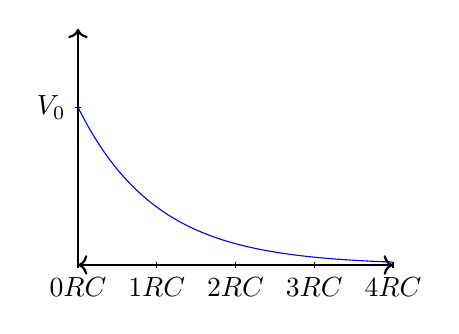
\begin{tikzpicture}
        \draw[thick,<->] (0,0) -- (4,0);
        \draw[thick,->] (0,0) -- (0,3);
        \foreach \x in {0, 1, 2, 3, 4}
            \draw (\x ,1pt) -- (\x ,-1pt) node[anchor=north] {$\x RC$};
        \foreach \y in {2}
            \draw (1pt,\y cm) -- (-1pt,\y cm) node[anchor=east] {$V_0$};
            \draw[scale=1,domain=0:4,smooth,variable=\x,blue] plot (\x,{2 * e^(-\x)});
    \end{tikzpicture}
\end{center}
Notice how the voltage decays to zero after a long time.
Now let's consider how a capacitor charges up.
\begin{figure}[H]
    \centering
        \begin{circuitikz} \draw
            (0,0) to[battery, l=$V$] (0,-4)
            (0, 0) to [capacitor, l=$V_C$, i=$i_C$] (4, 0)
            (4, 0) to[resistor, l=R, i=$i_R$] (4, -4) 
            to[switch, n=switch] (0, -4)
            (switch) node[above] {$t=0$};
        \end{circuitikz}
    \caption{A capacitor charging}
    \label{}
\end{figure}
At time $t=0$, the switch closes and currents start flowing to charge the capacitor.
As we did for the discharging capacitor, lets apply nodal analysis.
\[
    \begin{array}{c}
        V - V_C - i_CR = 0\\\\
        RC\frac{dV_c}{dt} = V - V_C\\\\
        \frac{dV_c}{dt} = \frac{1}{RC}(V-V_C)
    \end{array}
\]
This equation looks different from the earlier one, but we can solve it in the same way if we just change variables.
Let $z = V-V_C$.
\[
    \begin{array}{c}
        \frac{dz}{dt} = -\frac{dV_C}{dt}\\\\
        \therefore -\frac{dz}{dt} = \frac{1}{RC}z\\\\
        \frac{dz}{dt} = -\frac{1}{RC}z
    \end{array}
\]
This is the same differential equation we saw before, so $z = ce^{-\frac{t}{RC}}$.
At $t=0$, the capacitor is uncharged, so $V_C=0$, thus $z = V$ at $t=0$. This means $c = V$.
Now we can change variables back to get $V_C$
$$ Ve^{-\frac{t}{RC}} = V - V_C$$
$$ V_C = V(1 - e^{-\frac{t}{RC}}) $$
Looking at a graph of this tells us how the capacitor charges up.
\begin{center}
    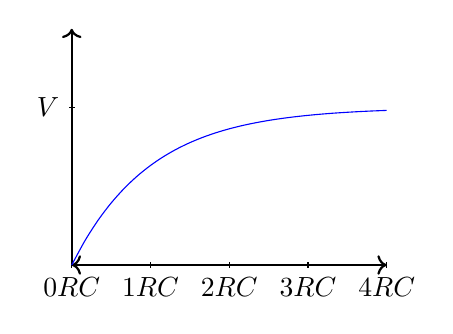
\begin{tikzpicture}
        \draw[thick,<->] (0,0) -- (4,0);
        \draw[thick,->] (0,0) -- (0,3);
        \foreach \x in {0, 1, 2, 3, 4}
            \draw (\x ,1pt) -- (\x ,-1pt) node[anchor=north] {$\x RC$};
        \foreach \y in {2}
            \draw (1pt,\y cm) -- (-1pt,\y cm) node[anchor=east] {$V$};
            \draw[scale=1,domain=0:4,smooth,variable=\x,blue] plot (\x,{2 * (1 - e^(-\x))});
    \end{tikzpicture}
\end{center}
Over time, the voltage on the capacitor takes on the voltage of the battery.
The time it takes for capacitors to charge and discharge explain why there are limits to how fast computers can work.
Remember that part of the transistor model contains a capacitor, so the time it takes for the capacitor to charge up limits how fast the transistor can switch between logic 0 and logic 1.
\subsection{RL Circuits}
Another circuit element which is commonly used in circuits is the inductor. The inductor tries to oppose changes in voltage.
Its IV relationship is $V = L\frac{dI}{dt}$ where $L$ is a constant called the inductance.
\\\\The analysis of inductors is the same as capacitors, but the behaviors are flipped.
\begin{figure}[H]
    \centering
        \begin{circuitikz} \draw
            (0,0) to[battery, l=$V$] (0,-4)
            (0, 0) to [inductor, l=$V_L$, i=$i_L$] (4, 0)
            (4, 0) to[resistor, l=R] (4, -4) 
            to[switch, n=switch] (0, -4)
            (switch) node[above] {$t=0$};
        \end{circuitikz}
    \caption{}
    \label{}
\end{figure}
\[
    \begin{array}{c}
        V - V_L - i_LR = 0\\\\
        V - L\frac{dI_L}{dt} - i_LR = 0\\\\
        \frac{dI_L}{dt} = \frac{V_s-i_LR}{L}
    \end{array}
\]
Solving this equation yields $I_L = I_0(1-e^{-\frac{Rt}{L}})$ where $I_0$ is the maximum current.
Notice how this is the same behavior that a capacitor exhibits but for the current instead.
\\\\Another easy comparison that can be made between inductors and capacitors is the energy stored in them.
The energy in a capacitor $U = \frac{1}{2}CV^2$, whereas the energy in an inductor is $\frac{1}{2}LI^2$.
\section{Frequency Analysis}
Solving differential equations is incredibly difficult, and for complex circuits, it is difficult to 
account for all the variables which are changing and to actually solve the differential equations.
Moreover, if we stop using DC inputs and instead use AC inputs, the time domain analysis becomes even more complicated.
\\\\To deal with this issue and to analyze more complex circuits, it becomes easier to analyze the "frequency response" of a circuit.
In other words, how does it respond to inputs of different frequencies.
\subsection{Phasor Representation}
Let's start by analyzing how a simple resistor circuit responds to different frequency voltages.
\begin{center}
    \begin{circuitikz} \draw
        (0,0) to[sV, l=$V$] (0,-4) -- (4, -4)
        (4, 0) to[resistor, l=R, i=$i_R$] (4, -4)
        (4, 0) -- (0, 0);
    \end{circuitikz}
\end{center}
Our input to this circuit is $V(t) = V_0cos(\omega t + \theta)$. Using Euler's formula, we can represent this as $V(t) = \frac{V_0}{2}e^{j\theta}(e^{j\omega t}+e^{-j\omega t})$.
Notice how $e^{-j\omega t}$ is the complex conjugate of $e^{j\omega t}$, which means if we know the angular frequency $\omega$, all of the "information" in the input
is described by the term $\frac{V_0}{2}e^{j\theta}$ (i.e we have both the amplitude and the phase of the signal encoded into a single complex number).
This encoding is known as a phasor, and lets call it $\tilde{V} = \frac{V_0}{2}e^{j\theta}$.
\begin{definition}
    A phasor encodes both the amplitude and phase of a sinusoidal input to a circuit.
\end{definition}
Notice that we can do normal circuit analysis with phasors. For example, the current in this circuit is $I = V/R = \frac{V_0}{R}V_0cos(\omega t + \theta)$. 
It's phasor representation is $\tilde{I} = \frac{V_0}{2R}e^{j\theta}$. This is exactly what we would get if we applied Ohm's law on the phasor $\tilde{V}$ (i.e, $\tilde{V} = \tilde{I}R$)
\subsection{Impedance}
In the time domain, the relationship between the voltage and current is the resistance. In the frequency domain, we define a more general concept called Impedance.
\begin{definition}
    The Impedance $Z$ of a circuit element is the ratio between the voltage phasor $\tilde{V}$ and the current phasor $\tilde{I}$.
    $$Z = \frac{\tilde{V}}{\tilde{I}}$$
\end{definition}
\subsubsection{Impedance of a Resistor}
Recall that for the simple resistor circuit above, $\tilde{V} = \frac{V_0}{2}e^{j\theta}$ and $\tilde{I} = \frac{V_0}{2R}e^{j\theta}$.
Thus the impedance $Z = \frac{\tilde{V}}{\tilde{I}} = R$. So for a resistor, the impedance is equivalent to the resistance ($Z = R$).
\subsubsection{Impedance of a Capacitor}
\begin{center}
    \begin{circuitikz} \draw
        (0,0) to[sV, l=$V$] (0,-4) -- (4, -4)
        (4, 0) to[capacitor, l=C, i=$i_C$] (4, -4)
        (4, 0) -- (0, 0);
    \end{circuitikz}
\end{center}
Now lets find the impedance of a capacitor.
$V = V_0cos(\omega t + \theta)$, so $\tilde{V} = \frac{V_0}{2}e^{j\theta}$ hasn't changed.
$$i_c = C\frac{dV}{dt} = -C\omega V_0sin(\omega t + \theta)$$
Since $sin(\omega t + \theta) = \frac{1}{2j}(e^{j\omega t}-e^{j\omega t})$
$$\tilde{I} = \frac{-C\omega V_0}{2j}e^{j\theta} = -C\omega V_0 je^{j\theta}$$
Now we can compute the impedance
$$Z = \frac{\tilde{V}}{\tilde{I}} = \frac{1}{j\omega C}$$
This is the impedance of the capacitor.
\subsubsection{Impedance of an Inductor}
\begin{center}
    \begin{circuitikz} \draw
        (0,0) to[sV, l=$I$] (0,-4) -- (4, -4)
        (4, 0) to[inductor, l=L, i=$i_L$] (4, -4)
        (4, 0) -- (0, 0);
    \end{circuitikz}
\end{center}
Let's do the same analysis for the inductor. Here our input signal is $I = I_0cos(\omega t + \theta)$.
That means $\tilde{I} = \frac{I_0}{2}e^{j\theta}$.
$$V = L\frac{dI}{dt} = -LI_0\omega sin(\omega t + \theta)$$
$$\tilde{V} = -\frac{LI_0\omega}{2j}e^{j\theta} = -\frac{LI_0\omega j}{2}e^{j\theta}$$
$$Z = \frac{\tilde{V}}{\tilde{I}} = j\omega L$$
This is the impedance of the inductor.
\subsection{Phasor Analysis}
Now that we know the impedances of different circuit components, we can start to analyze circuits with them.
Consider this RC circuit
\begin{center}
    \begin{circuitikz} \draw
        (0,0) to[sV, l=$V$] (0,-4)
        (0, 0) to [resistor, l=R] (4, 0)
        (4, 0) to[capacitor, l=$V_C$] (4, -4) 
        (4, 0) to[short, -o] node[right] {$V_{out}$} (5, 0)
        (0, -4) node[ground] {}
        (4, -4) node[ground] {};
    \end{circuitikz}
\end{center}
If we wanted to find $V_{out}$, we could write out the differential equations and solve, but with phasors, everything becomes easier.
First we convert everything to the phasor domain. Sinusoidal inputs become DC inputs, and resistors, capacitors, and inductors become impedances.
\begin{center}
    \begin{circuitikz}[european resistors] \draw
        (0,0) to[battery, l=$\tilde{V}$] (0,-4)
        (0, 0) to [resistor, l=R] (4, 0)
        (4, 0) to[resistor, l=$\frac{1}{j\omega C}$] (4, -4) 
        (4, 0) to[short, -o] node[right] {$\tilde{V}_{out}$} (5, 0)
        (0, -4) node[ground] {}
        (4, -4) node[ground] {};
    \end{circuitikz}
\end{center}
This is just a voltage divider, so 
$$\tilde{V}_{out} = \frac{\frac{1}{j\omega C}}{R + \frac{1}{j\omega C}}\tilde{V} = \frac{1}{1 + j\omega RC}\tilde{V}$$
Lets define $H(\omega) = \frac{1}{1 + j\omega RC}$, so $\tilde{V}_{out} = H(\omega)\tilde{V}$
Now if our original signal was $V = cos(\omega t)$, then $\tilde{V} = \frac{1}{2}$, so $\tilde{V}_{out} = \frac{1}{2}H(\omega)$.
To convert this back into the time domain, we know the phasor is encoding some sinusoidal signal,
so $$V_{out} = \tilde{V}_{out}e^{j\omega t}+\tilde{V}_{out}e^{-j\omega t} = \frac{1}{2}|H(\omega)|cos(\omega t + \angle H(\omega))$$
Thus we have recovered our output signal using no calculus.
\subsection{Transfer Functions}
Notice how in the previous example, the relationship between our "output" $\tilde{V}_{out}$ and our input $\tilde{V}$ was described by a function $H(\omega)$.
This function is called the transfer function.
\begin{definition}
    The Transfer Function of a circuit is defined as $H(\omega) = \frac{\tilde{X}}{\tilde{V}}$ where $\tilde{X}$ 
    is the phasor output and $\tilde{V}$ is the phasor input
\end{definition}
The transfer function gives us a convenient way to analyze how a circuit will affect an input signal depending on its angular frequency, effectively treating the circuit like a black box.
An important note is that transfer functions do not just apply to voltages, they can also apply to currents, but for the most part, we will deal with voltages.
\\\\All transfer functions can be expressed in the form $H(\omega) = \frac{Z(\omega)}{P(\omega)}$. $Z(\omega)$ and $P(\omega)$ are complex polynomials.
If we factor $P(\omega)$ and $Z(\omega)$, then we see that all transfer functions can be expressed as follows.
$$H(\omega) = \frac{(j\omega)^{N_{z0}}}{(j\omega)^{N_{p0}}} \frac{\prod_{z=0}^{n}{(j\omega)^z \alpha_z}}{\prod_{p=0}^{m}{(j\omega)^p \beta_p}} = K \frac{(j\omega)^{N_{z0}}}{(j\omega)^{N_{p0}}}\frac{\prod_{i=0}^{n}{(1+\frac{j\omega}{\omega_{zi}})}}{\prod_{k=0}^{m}{(1+\frac{j\omega}{\omega_{pk}})}}$$
The constants $\omega_z$ are the zeros of the complex polynomial $Z(\omega)$, and the constants $\omega_p$ are the series of the complex polynomial $P(\omega)$.
$\omega_z$ are called the zeros of the transfer function, and $\omega_p$ are called the poles.
$N_{z0}$ and $N_{p0}$ are the number of zeros and poles respecively at $\omega=0$.
\\\\To see how this makes analysis easier, lets look at the transfer function we saw earlier $H(\omega) = \frac{1}{1 + j\omega RC}$.
We can rewrite $H(\omega) = \frac{1}{1+\frac{\omega}{\omega_p}}$, where $\omega_p = \frac{1}{RC}$.
Notice how when $\omega >> \omega_p$, $H(\omega) \approx 0$ and when $\omega << \omega_p, H(\omega) \approx 1$.
This tells us that for frequencies higher than the pole, the input will be attenuated, but for frequencies less than the pole, the signal will be mostly unaffected.
\subsection{Bode Plots}
For more complex transfer functions, we need a easier way of analyzing them than taking limits. This is where Bode Plots come in.
\begin{definition}
    A Bode Plot is a plot of $|H(\omega)|$ and $\angle H(\omega)$ on a log-log scale
\end{definition}
These visually reveal the behavior of circuits. The log-log scale not only allows us to determine the behavior of Bode plots over a large range of frequencies,
but they also let us easily figure out what the plot looks like because it converts the transfer function into piecewise linear components.
\\\\To see why, lets write our transfer function in polar form. 
$$H(\omega) = K \frac{(j\omega)^{N_{z0}}}{(j\omega)^{N_{p0}}}\frac{\prod_{i=0}^{n}{(1+\frac{j\omega}{\omega_{zi}})}}{\prod_{k=0}^{m}{(1+\frac{j\omega}{\omega_{pk}})}} = Ke^{j\frac{\pi}{2}(N_{z0}-N_{p0})} \frac{\prod_{i=0}^{n}{r_{zi}}}{\prod_{k=0}^{m}{r_{pk}}} e^{j(\sum_{i=0}^{n}{z_i} - \sum_{k=0}^{m}{p_k})}$$
Each $r$ is the magnitude of a factor $1 + \frac{j\omega}{\omega_n}$ where $\omega_n$ is either a root or a pole, and the $z_i, p_k$ are the phases of each factor.
By writing $H(\omega)$ this way, it is clear that $$|H(\omega)| = K \frac{\prod_{i=0}^{n}{r_{zi}}}{\prod_{k=0}^{m}{r_{pk}}}$$
If we take the log of this, we get $$log(|H(\omega)|) = log(K) + \sum_{i=0}^{n}{log(r_{zi})} - \sum_{k=0}^{m}{log(r_{pk})}$$
Likewise, the exponential form of $H(\omega)$ tells us that $$\angle H(\omega) = \frac{\pi}{2}(N_{z0}-N_{p0})+ (\sum_{i=0}^{n}{z_i} - \sum_{k=0}^{m}{p_k})$$
Next, we should verify if we can approximate these equations as linear on a log-log scale.
Take the example transfer function $H(\omega) = \frac{1}{1+\frac{j\omega}{\omega_p}} = \frac{1}{r_p}e^{-j\theta_p}$.
\[
    \begin{array}{cccc}
        \text{if } \omega = \omega_p & H(\omega) = \frac{1}{1+j} & r_p = \sqrt{2} & \theta_p = \frac{\pi}{4}\\
        \text{if } \omega = 10\omega_p & H(\omega) = \frac{1}{1+10j} & r_p \approx 10 & \theta_p \approx \frac{\pi}{2}\\
        \text{if } \omega = 0.1\omega_p & H(\omega) = \frac{1}{1+0.1j} & r_p \approx 1 & \theta_p \approx 0\\
    \end{array}
\]
Thus we can see at decades away from the poles and zeros, the magnitudes and the phases will have less of an effect.
Let's try constructing the Bode Plot for this transfer function.
\begin{center}
    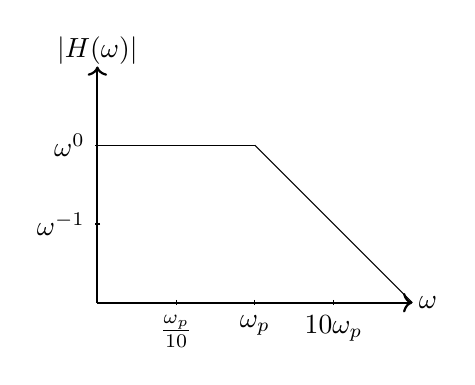
\begin{tikzpicture}
        \draw[thick,->] (0,0) -- (4,0);
        \draw[thick,->] (0,0) -- (0,3);
        \draw (4.2, 0) node[] {$\omega$};
        \draw (0, 3.2) node[] {$|H(\omega)|$};
        \draw(1, 1pt) -- (1, -1pt) node[anchor=north] {$\frac{\omega_p}{10}$};
        \draw(2, 1pt) -- (2, -1pt) node[anchor=north] {$\omega_p$};
        \draw(3, 1pt) -- (3, -1pt) node[anchor=north] {$10\omega_p$};
        \draw (1pt,2 cm) -- (-1pt,2 cm) node[anchor=east] {$\omega^0$};
        \draw (1pt,1 cm) -- (-1pt,1 cm) node[anchor=east] {$\omega^{-1}$};
        \draw (0, 2cm) -- (2, 2cm);
        \draw (2, 2cm) -- (4, 0cm);
    \end{tikzpicture}
    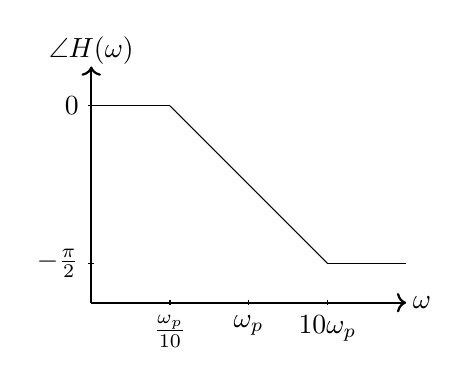
\begin{tikzpicture}
        \draw[thick,->] (0,0) -- (4,0);
        \draw (4.2, 0) node[] {$\omega$};
        \draw (0, 3.2) node[] {$\angle H(\omega)$};
        \draw[thick,->] (0,0) -- (0,3);
        \draw(1, 1pt) -- (1, -1pt) node[anchor=north] {$\frac{\omega_p}{10}$};
        \draw(2, 1pt) -- (2, -1pt) node[anchor=north] {$\omega_p$};
        \draw(3, 1pt) -- (3, -1pt) node[anchor=north] {$10\omega_p$};
        \draw (1pt,2.5 cm) -- (-1pt,2.5 cm) node[anchor=east] {$0$};
        \draw (1pt,0.5 cm) -- (-1pt,0.5 cm) node[anchor=east] {$-\frac{\pi}{2}$};
        \draw (0, 2.5cm) -- (1, 2.5cm);
        \draw (1, 2.5cm) -- (3, 0.5cm);
        \draw (3, 0.5cm) -- (4, 0.5cm);
    \end{tikzpicture}
\end{center}
For the magnitude plot, since there are no poles or zeros at $\omega = 0$, we draw a straight line until the pole kicks in at $\omega = \omega_p$ at which point the slope of the line will be -1.
For the phase plot, we apply the same logic, except the pole kicks in at $\frac{\omega_p}{10}$ (to see why, look above to see how at $\omega = \omega_p$, the phase is $-\frac{\pi}{4}$).
We can apply this same logic for more complicated transfer functions too.
Lets take $$H(\omega) = 10^9 \frac{(1+\frac{j\omega}{10^9})}{(j\omega)(1+\frac{j\omega}{10^7})}$$
Notice we have a zero at $10^9$, poles at $1, 10^7$, and 9 zeros at $\omega = 0$. With this information, we can see the plots will look like this:
\begin{center}
    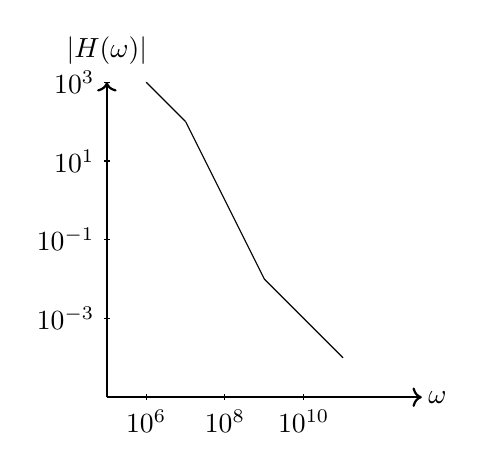
\begin{tikzpicture}
        \draw[thick,->] (0,0) -- (4,0);
        \draw[thick,->] (0,0) -- (0,4);
        \draw (4.2, 0) node[] {$\omega$};
        \draw (0, 4.4) node[] {$|H(\omega)|$};
        \draw(0.5, 1pt) -- (0.5, -1pt) node[anchor=north] {$10^6$};
        \draw(1.5, 1pt) -- (1.5, -1pt) node[anchor=north] {$10^8$};
        \draw(2.5, 1pt) -- (2.5, -1pt) node[anchor=north] {$10^{10}$};
        \draw (1pt,4) -- (-1pt,4) node[anchor=east] {$10^3$};
        \draw (1pt,3) -- (-1pt,3) node[anchor=east] {$10^1$};
        \draw (1pt,2) -- (-1pt,2) node[anchor=east] {$10^{-1}$};
        \draw (1pt,1) -- (-1pt,1) node[anchor=east] {$10^{-3}$};
        \draw (0.5, 4) -- (1, 3.5);
        \draw (1, 3.5) -- (2, 1.5);
        \draw (2, 1.5) -- (3, 0.5);
    \end{tikzpicture}
    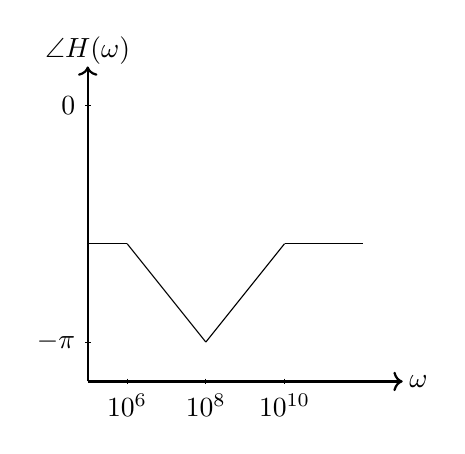
\begin{tikzpicture}
        \draw[thick,->] (0,0) -- (4,0);
        \draw (4.2, 0) node[] {$\omega$};
        \draw (0, 4.2) node[] {$\angle H(\omega)$};
        \draw[thick,->] (0,0) -- (0,4);
        \draw(0.5, 1pt) -- (0.5, -1pt) node[anchor=north] {$10^6$};
        \draw(1.5, 1pt) -- (1.5, -1pt) node[anchor=north] {$10^8$};
        \draw(2.5, 1pt) -- (2.5, -1pt) node[anchor=north] {$10^{10}$};
        \draw (1pt,3.5 cm) -- (-1pt,3.5 cm) node[anchor=east] {$0$};
        \draw (1pt,0.5 cm) -- (-1pt,0.5 cm) node[anchor=east] {$-\pi$};
        \draw (0, 1.75cm) -- (0.5, 1.75cm);
        \draw (0.5, 1.75cm) -- (1.5, 0.5cm);
        \draw (1.5, 0.5cm) -- (2.5, 1.75cm);
        \draw (2.5, 1.75cm) -- (3.5, 1.75cm);
    \end{tikzpicture}
\end{center}
The pole at 0 kicks in immediately, causing the decreasing magnitude and starting the phase at $\frac{-\pi}{2}$. The second pole at $10^7$ will kick in next, followed by the zero at $10^9$.
\subsection{Filters}
One type of circuit which Bode plots make very easy to analyze are filters.
\subsubsection{Low Pass Filters}
\begin{definition}
    A low pass filter is one which allows frequencies below a particular cutoff frequency to pass through while higher ones are attenuated.
\end{definition}
Two common low pass filters are the RC filter and the LR filter.
\begin{figure}[H]
    \centering
        \begin{circuitikz} \draw
            (0, 0) node[left] {$\tilde{V}_{in}$} to[resistor, o-o, l=R] 
            (3, 0) node[right] {$\tilde{V}_{out}$}
            (2.5, 0) to[capacitor, l=C] (2.5, -2) node[ground] {};
        \end{circuitikz}
        \begin{circuitikz} \draw
            (0, 0) node[left] {$\tilde{V}_{in}$} to[inductor, o-o, l=L] 
            (3, 0) node[right] {$\tilde{V}_{out}$}
            (2.5, 0) to[resistor, l=R] (2.5, -2) node[ground] {};
        \end{circuitikz}
    \caption{Low Pass Filters}
    \label{}
\end{figure}
These both have the transfer function $H(\omega) = \frac{1}{1+\frac{j\omega}{\omega_p}}$ where $\omega_p = \frac{1}{RC}$ or $\omega_p=\frac{R}{L}$ depending on which filter it is.
In this case, $\omega_p$ is called the cutoff frequency.
\subsubsection{High Pass Filters}
\begin{definition}
    A high pass filter is on which allows frequencies higher than a particular cutoff frequency to pass through while lower ones are attenuated.
\end{definition}
Two common high pass filters are the RL and CR filters.
\begin{figure}[H]
    \centering
        \begin{circuitikz} \draw
            (0, 0) node[left] {$\tilde{V}_{in}$} to[capacitor, o-o, l=C] 
            (3, 0) node[right] {$\tilde{V}_{out}$}
            (2.5, 0) to[resistor, l=R] (2.5, -2) node[ground] {};
        \end{circuitikz}
        \begin{circuitikz} \draw
            (0, 0) node[left] {$\tilde{V}_{in}$} to[resistor, o-o, l=R] 
            (3, 0) node[right] {$\tilde{V}_{out}$}
            (2.5, 0) to[inductor, l=L] (2.5, -2) node[ground] {};
        \end{circuitikz}
    \caption{High Pass Filters}
    \label{}
\end{figure}
These both have the transfer function $H(\omega) = \frac{j\omega}{1+\frac{\omega}{\omega_p}}$
where $\omega_p = \frac{1}{RC}$ or $\omega_p=\frac{R}{L}$ depending on which filter it is.
Once again, $\omega_p$ is called the cutoff frequency.
\subsubsection{LC Tank}
\begin{definition}
    The LC tank is an inductor and a capacitor in series. When the input is at the resonating frequency, these act like an infinite impedance.
\end{definition}
\begin{figure}[H]
    \centering
        \begin{circuitikz} \draw
            (0, 0) node[left] {$\tilde{V}_{in}$} to[capacitor, o-o, l=C] 
            (3, 0) node[right] {$\tilde{V}_{out}$}
            (2.5, 0) to[inductor, l=L] (2.5, -2) node[ground] {};
        \end{circuitikz}
    \caption{LC Tank}
    \label{}
\end{figure}
The transfer function $H(\omega) = \frac{j\omega L}{j\omega L + \frac{1}{j\omega C}}$. If $\omega = \omega_n = \sqrt{\frac{1}{LC}}$, 
then this transfer function gets infinitely large effectively acting like an infinite impedance. $\omega_n$ is called the resonant frequency.
\section{Discrete Time Models}
Although circuits and other systems function in continuous time, computers can only act in discrete time.
This means the signals they send out to try and control the system are piecewise-continuous, and they can only sense the system at specified intervals $\delta$.
At a discrete time-step $i$, the computer will measure $\vec{x}_d[i]$ and applies the control $\vec{u}[i]$ over the time-interval $[i, i+1]$.
Keep in mind that $i=\delta t$ where $t$ is the continuous time.
\begin{definition}
    The discrete-time state space model is $\vec{x}_d[i+1]=A_d\vec{x}_d[i]+B_d\vec{u}[i]+\vec{w}[i]$ where $\vec{w}[i]$ is some disturbance.
\end{definition}
\subsection{Converting between continuous time and discrete time}
To see how to convert between a continuous time model to a discrete time model, consider the following system.
\[
    \begin{array}{c}
        \frac{dx}{dt}=\lambda x+u, u=e^{st}\\
        \left(
            \frac{d}{dt}-\lambda
            \right)x = u
    \end{array}\\
\]

Solving will give $x=\alpha e^{\lambda t}+\beta e^{st}$
Plugging this into the original equation
\[
    \begin{array}{c}
        \alpha \lambda e^{st}+\beta se^{st} = \lambda (\alpha e^{\lambda t}+\beta e^{st})+e^{st}\\
        \text{if}\> \lambda \ne s\\
        \beta s = \beta \lambda + 1 \implies \beta = \frac{1}{s-\lambda}
    \end{array}
    \]
Since the computer only outputs constant signals, $s=0$, so $x=\alpha e^{\lambda t}-\frac{u}{\lambda}$
If $x(0)=x_0$
\[
    \begin{array}{c}
        x(0)=\alpha - \frac{u}{\lambda}=x_0\\
        x = (x_0+\frac{u}{\lambda}e^{\lambda t})-\frac{u}{\lambda}\\
        x = x_0 e^{\lambda t}+u\left(
            \frac{e^{\lambda t}-1}{\lambda}
        \right)
    \end{array}
\]

Thus the discrete time model is
$$x[i+1]=e^{\lambda \delta}x[i]+\left(
    \frac{e^{\lambda \delta}-1}{\lambda}\right) u[i]$$
since the initial condition for the next time-step is simple the value at the previous time-step

\subsection{Finding A and B}
What would happen if we didn't know what A and B were though? It turns out that we can find it by gathering data about the system and then using least squares.
In the scalar case:
\[
    \begin{array}{c}
        x[i+1]=ax[i]+bu[t]+w[i]\\
        x[1]=ax[0]+bu[0]\\
        x[2]=ax[1]+bu[1]\\
        \vdots\\
        x[m]=ax[m-1]+bu[m-1]
    \end{array}
\]
This means with $m$ observations, we can construct a matrix $D$ and a vector $\vec{s}$ such that we have the least squares problem
\[
    D\vec{p}=\vec{s},\text{ where } \vec{p}=
\left[
    \begin{array}{c}
        a\\
        b\\
    \end{array}
\right]
\]
The same thing can be done in the vector case. We just create multiple parallel systems by multiplying out the rows.
\section{Control Theory}
\subsection{Controllability}
\begin{definition}
    A system is controllable if $\forall x^*, \forall x[0], \exists u[0],u[1],...,u[k-1]$ such that $x[k]=x^*$ given that the system starts at $x[0]$
\end{definition}
In words, this means that there exists a sequence of control actions that can eventually get the system anywhere we want it to be from any given initial state.
\begin{theorem}
    If a state is n-dimensional, then a system $\vec{x}_d[i+1]=A\vec{x}[i]+B\vec{u}[i]+\vec{w}[i]$ is controllable in k time-steps if $span(B, AB, ..., A^{k-1}B)=\mathbb{R}^n$
\end{theorem}
\begin{proof}
    Without any noise, $\vec{x}_d[i+1]=A\vec{x}[i]+B\vec{u}[i]$
    \[
        \begin{array}{c}
            \vec{x}[1]=A\vec{x}[0]+B\vec{u}[0]\\
            \vec{x}[2]=A\vec{x}[1]+B\vec{u}[1] = A^2\vec{x}[0]+AB\vec{u}[0]+B\vec{u}[i]\\
            \vec{x}[3]=A\vec{x}[2]+B\vec{u}[2] = A^3\vec{x}[0]+A^2B\vec{u}[0]+AB\vec{u}[i]+B\vec{u}[2]\\
            \vdots\\
            \vec{x}[k]=A^k\vec{x}[0]+\sum_{i=0}^{k-1}{A^{k-i-1}B\vec{u}[i]}
        \end{array}
        \]
    Thus the current state is merely a linear combination of vectors in the column spaces of $A^k$ and $B...A^{k-1}$, so if this span is equal to $\mathbb{R}^n$, we can reach every state.
\end{proof}
\begin{definition}
    The controllability matrix is a the matrix whose column space is all the reachable states.
    \[
        \mathcal{C} = \left[
            \begin{array}{c|c|c|c|c}
                B & AB & A^2B & ... & A^{k-1}B
            \end{array}
        \right]
        \]
\end{definition}
However, if we want to check if a system is controllable in 100 time-steps for a 100 state system, it will be painful to calculate the column space of the controllability matrix.
It turns out that we can stop checking when $dim(col(B, AB,...,A^{p-1}))=dim(col(B, AB, ..., A^p)), (p \leq k)$ (i.e the dimension of the column space stops growing)
This means we can build the controllability matrix up piece-by-piece and stop early rather than computing the full column space only to fail. Consider the following proof for why this works.
\begin{proof}
    If $\vec{b}$ is column vector of the matrix B, then $A^p \vec{b}=\sum_{i=0}^{p-1}{\alpha_iA^i\vec{b}}$ since we assume the dimension of the column space has stopped growing,
    so $A^p\vec{b}$ is a linear combination of the vectors preceding it.
    We want to show $\exists \beta_i$ such that $A^{p+1}=\sum_{i=0}^{p-1}{\beta_iA^i\vec{b}}$
    \[
        \begin{array}{c}
            A^{p+1}\vec{b}=A(A^p\vec{b}) =\\
            A\sum_{i=0}^{p-1}{\alpha_iA^i\vec{b}} = \sum_{i=0}^{p-1}{\alpha_iA^{i+1}\vec{b}}=\\
            \alpha_{p-1}A^p\vec{b}+ \sum_{i=0}^{p-2}{\alpha_iA^{i}\vec{b}}=\\
            \alpha_{p-1}\sum_{i=0}^{p-1}{\alpha_iA^i\vec{b}}+\sum_{i=0}^{p-2}{\alpha_iA^{i}\vec{b}}
        \end{array}
        \]
    By writing $A^{p+1}$ as a linear combination of $B, AB,...,A^{p-1}$, we have shown $\beta_i$ exists, so by induction, all future vectors $p+m\leq k$ will be linear combinations of these same vectors, 
    so the dimension will never grow again and we can be justified in stopping early.
\end{proof}
\subsection{Observability}
Another question we can ask about different systems is whether or not we can figure out exactly where we are.
Often times, we are limited in the measurements we can take, and so we might not be able to "see" the entire state vector $\vec{x}[t]$.
Instead, we would only be able to see the output $\vec{y}[t]=C\vec{x}[t]$. To start with, consider what would happen if we applies no inputs to the system.
\[
    \begin{array}{c}
        \vec{y}[0] = C\vec{x}[0]\\
        \vec{y}[1] = C\vec{x}[1] = CA\vec{x}[0]\\
        \vdots\\
        \vec{y}[n] = CA^n\vec{x}[0]\\
    \end{array}
\]
If we want to recover the state $\vec{x}[0]$, we could apply least squares.
$$\vec{x}[0] = (\mathcal{O}^T\mathcal{O}^{-1}\mathcal{O}^T\vec{y}$$
where
\[
    \mathcal{O} = \left[
        \begin{array}{c}
            C\\
            CA\\
            \vdots\\
            CA^i
        \end{array}
    \right],\ \vec{y} = \left[
        \begin{array}{c}
            \vec{y}[0]\\
            \vec{y}[1]\\
            \vdots\\
            \vec{y}[n]\\
        \end{array}
        \right]
\]
$\mathcal{O}$ is known as the observability matrix, and we can use least squares as long as it is full rank.
\begin{theorem}
    A system is observable if $\mathcal{O}$ has linearly independent columns.
\end{theorem}
Even if a system has inputs, this kind of analysis still holds.
Define 
$$\vec{x}_f[i]=A\vec{x}[i],\ \vec{y}_f[i]=C\vec{x}_f[0]$$
This is what the system would do without any inputs. If we unroll the recursion in the system, we see
\[
    \begin{array}{c}
        \vec{x}[i] = \vec{x}_f[i]+\sum_{k=0}^{i-1}{A^{i-k-1}B\vec{u}[k]}\\\\
        \vec{y}[i] = \vec{y}_f[i]+\sum_{k=0}^{i-1}{CA^{i-k-1}B\vec{u}[k]}
    \end{array}
\]
Since we know the inputs we applied, and $\vec{x}_f[i]=A^i\vec{x}[i]$, we can easily find $\vec{x}_f[i],\ \vec{y}_f[i]$
and then apply least squares to them to compute the initial state.

\subsection{Stability}
The question of stability is whether or not disturbances will over time control a system if left alone.
Specificically, it is asking if the disturbances are bounded, will the states be bounded too?
\begin{definition}
    Bounded Input, Bounded Output (BIBO) stability means if $|\vec{w}[i| < \epsilon$, then $\exists \delta>0$ such that $|\vec{x}[i| < \delta$
\end{definition}

To see where this definition comes into play, consider the following scalar systems:
\begin{itemize}
    \item[1.] $x[i+1] = u[i] + w[i]$
    \item[2.] $x[i+1] = \frac{1}{2}x[i] + u[i]+w[i]$ ("Weak" dependence on previous state)
    \item[3.] $x[i+1] = 2 x[i]+u[i]+w[i]$ ("Strong" dependence on previous state)
\end{itemize}
\begin{itemize}
    \item[System 1:] In this system, there is no dependence on the previous state.
    Thus any disturbances are limited to affecting only the next state and no others.
    This makes the system stable because disturbances will not add up.
    To see this mathematically, pretend $u[i] = 0$ since we want to see how the system evolves without doing anything.
    $$|x[i+1]|=|w[i]| < \epsilon, \>\>\> \therefore |x[i]|<\epsilon$$
    Thus we have BIBO stability
    \item[System 2:] Unlike the previous system, this system has a "weak" dependence on previous states. We consider it "weak" because only half of the previous state influences the next state.
    Intuitively, this system must be BIBO stability then because although disturbances will accumulate, they will be attenuated through an infinite geometric sum. Once again, we will pretend $\vec{u}[i]=0$ to check this mathematically.
    $$|x[i+1]| = \frac{1}{2}x[i]+w[i] < \frac{1}{2}x[i]+ \epsilon$$
    Unrolling the recursive relationship, we see
    $$|x[i+1]| < \epsilon+\frac{1}{2}\epsilon+\frac{1}{4}\epsilon+...+\left( \frac{1}{2} \right)^i\epsilon$$
    $$\lim_{i->\infty}{|x[i+1]}<\frac{\epsilon}{1-\frac{1}{2}} = 2\epsilon$$
    Thus the system is BIBO stability since $|x[i]| < 2\epsilon$
    \item[System 3:] This system has a "strong" dependence on previous states since the contribution of previous states is doubled each times.
    Intuitively, this means the system must be unstable because small disturbances will be explode over time. To see this mathematically, once again consider what happens if we apply no inputs.
    $$|x[i+1]| = 2x[i]+w[i] < 2x[i]+ \epsilon$$
    Unrolling the recursion,
    $$|x[i+1]| < \epsilon+2\epsilon+4\epsilon+...+2^i\epsilon$$
    $$\lim_{i->\infty}{|x[i+1]} < \infty$$
    Thus $|x[i]|$ has no bound, so the system is not stable.
\end{itemize}

Note that in the scalar case, as long as $|\lambda| < 1$ for the system $x[i+1]=\lambda x[i]+bu[i]+w[i]$, the system will be stable. Note that this is $\lambda<1$, not $\lambda \leq 1$. That is because when $\lambda=1$, we can see the errors will add up.
It turns out that in the vector case, for the system $\vec{x}[t+1]=A \vec{x}[t]+B\vec{u}[t]+\vec{w}[t]$, the system will be stable if the eigenvalues of A are less than 1.
\begin{proof}
    If $\exists \> n \> \vec{v}_i$ such that $A\vec{v}_i=\lambda_i\vec{v}_i$, then changing coordinates to the eigenbasis gives
    $$\tilde{A}=
        \left[
        \begin{array}{ccc}
        \lambda_1 &  & 0 \\
         & \ddots &  \\
        0 &  & \lambda_n \\
        \end{array}
        \right] $$
    This means $\vec{\tilde{x}}[t+1]=\tilde{A}\vec{\tilde{x}}[t]+V^{-1}B\vec{u}[t]+V^{-1}\vec{w}[t]$ where $V$ is the matrix whose columns are A's eigenvectors.
    This is merely n different scalar cases, but we still have to make sure that $|\vec{w}[t]|<\epsilon \implies |V^{-1}\vec{w}[t]|<\kappa$ where $\kappa$ is some bound.
    Lets say $m=V_{ij}^{-1}$ is the largest entry in $V^{-1}$. In the worst case all $\vec{w}_i[t]$ and all $V_{ij}=m$.
    Then $\forall i, \left[V^{-1}\vec{w}[t]\right]_i \leq n m \epsilon$ where $n$ is the dimension of $V$, which means $|V^{-1}\vec{w}[t]|<\kappa$.
    Thus we can say that $\tilde{x}[t]$ is BIBO implies that $\vec{x}[t]$ is BIBO.
\end{proof}
It is important to realize that the condition $|\lambda|<1$ holds only for discrete-time systems. If instead our system is continuous (i.e $\frac{d}{dt}\vec{x}(t)=A\vec{x}(t)+B\vec{u}(t)$),
then the system will only be stable if $Re\{\lambda\}<0$. To see why, consider the following simple linear system with initial condition $x_0$.
\[
    \begin{array}{c}
        \frac{d}{dt}x(t) = \lambda x(t)\\
        \therefore x(t) = x_0 e^{\lambda t}
    \end{array}
\]
Clearly if $\lambda > 0$, this system will grow infinitely large. The same analysis applies to vector cases.
\subsubsection{Stability for a general A matrix}
Notice that checking stability based on the eigenvalues requires the matrix $A$ to be diagonalizable becase we need to check all of its eigenvalues.
This leaves open the question of what happens when $A$ is not diagonalizable, meaning there are not n distinct eigenvalues.
In order to resolve this problem, we are going to need a new matrix form called Shurr Upper Triangular Form
\begin{definition}
    The Shurr Upper Triangular form of a matrix A is
    \[
        \left[
            \begin{array}{cccc}
                \lambda_1 & * & * & ... \\
                0 & \lambda_2 & * & ... \\
                0 & 0 & \ddots & \\
                \vdots & \vdots &  & 
            \end{array}
        \right]
        \]
    It is an upper triangular matrix with eigenvalues on the diagonal. The eigenvalues may equal = 0.
\end{definition}
Shurr form allows us to easily find the characteristic polynomial of the matrix and solve the problem of stability.
To see why it helps with stability, consider the following proof.
\begin{proof}
    $$\tilde{x}[t+1]=\tilde{A}\tilde{x}[t]+\tilde{w}[t]$$
    If $\tilde{A}$ is in Shurr form, then the nth component is
    $$\tilde{x}_n[t+1]=\lambda_n\tilde{x}_n[t]+\tilde{w}_n[t]$$
    so if $|\lambda_n| < 1$, then $\tilde{x}_n$ is BIBO stable.
    Likewise, for the n-1th component
    $$\tilde{x}_{n-1}[t+1]=\lambda_{n-1}\tilde{x}_{n-1}[t]+s\tilde{x}_n[t]+\tilde{w}_{n-1}[t]$$
    $s$ is one of the $*$ entries in the upper part of Shurr form. It doesn't matter what it is because $\tilde{x}_n[t]$ is BIBO, so $s\tilde{x}_n[t]$ is also BIBO.
    As a result $$\tilde{x}_{n-1}[t]$$ will be BIBO if $|\lambda_{n-1}|<1$ and $|\lambda_n| < 1$.
    Since the component $\tilde{x}_{n-i}[t+1]$ depends on $\tilde{x}_n[t], \tilde{x}_{n-1}[t],...$, as long as $\tilde{x}_n[t], \tilde{x}_{n-1}[t],...$ are stable, $\tilde{x}_{n-i}[t+1]$ will be stable too.
    Thus as long as all $|\lambda_i|<1$, then Shurr form tells us whether or not the system is stable.
\end{proof}
Now that we know how it works, we need to know how to find a basis $U$ such that $\tilde{A}=U^{-1}AU$. As a bonus, it would be helpful if $U$ is orthonormal.
To make things easier later, we'll define $M_n = A$. Since all matrices have at least one eigenpair, we can choose
$$M\vec{v}_1=\lambda_1\vec{v}_1, ||\vec{v}_1||=1$$

Using Gram-Schmidt, we can now pick $n-1$ vectors $\vec{r}_i$ such that
$$U_1 = \vec{v}_1, \vec{r}_1, ..., \vec{r}_{n-1}$$ is an orthonormal basis. Note, the vectors $\vec{r}_i$ form a $n \times (n-1)$ matrix $R_{n-1}$
Lets look at $M_n$ in the $U_1$ basis.
\[
    U_1^{-1}M_nU_1=
    \left[
        \begin{array}{c}
            \vec{v}_1^T \\\\
            R_{n-1}^T
        \end{array}
    \right]
    M_n
    \left[
        \begin{array}{cc}
            \vec{v}_1 & R_{n-1}
        \end{array}
    \right] = 
    \left[
        \begin{array}{cc}
            \vec{v}_1^T M_n \vec{v}_1 & \vec{v}_1^T M_n R_{n-1} \\\\
            R_{n-1}^T M_n \vec{v}_1^T & R_{n-1}^T M_n R_{n-1}
        \end{array}
    \right] = 
    \left[
        \begin{array}{c|c}
            \lambda_1 & * \\
            \hline\\
            0 & R_{n-1}^T M R_{n-1}
        \end{array}
    \right]
\]
We can see that we are getting closer to where we want to be, so lets continue with the matrix $M_{n-1}$.
We can find a vector of size $n-1$ such that
$$M_{n-1}\vec{v_2}=\lambda_2\vec{v}_2, ||\vec{v}_2||=1$$
Extending this to an orthonormal basis $U_2$, we get a matrix $R_{n-2}$
\[
    \left[
        \begin{array}{c}
            \vec{v}_2^T \\\\
            R_{n-2}^T
        \end{array}
    \right]
    M_{n-1}
    \left[
        \begin{array}{cc}
            \vec{v}_2 & R_{n-2}
        \end{array}
    \right] = 
    \left[
        \begin{array}{cc}
            \vec{v}_2^T M_{n-1} \vec{v}_2 & \vec{v}_2^T M_{n-1} R_{n-2} \\\\
            R_{n-1}^T M_{n-1} \vec{v}_1^T & R_{n-1}^T M_{n-1} R_{n-1}
        \end{array}
    \right] = 
    \left[
        \begin{array}{c|c}
            \lambda_2 & * \\
            \hline\\
            0 & R_{n-2}^T M_{n-1} R_{n-2}
        \end{array}
    \right]
\]
We can keep repeating this by saying $M_{n-2} = R_{n-2}^T M_{n-1} R_{n-2}$, but we need to know if our $\lambda_2$ has any relation to the eigenvalues of A.
Lets say $$U_2 = \vec{v}_1, \vec{x}, rest$$ is a basis where $\vec{x}$ has some dependence on $\vec{v}_2$.
There aren't many options for what $\vec{x}$ and the rest of the basis vectors could be, so let's try.
$$\vec{x}=R_{n-1}\vec{v}_2,\ rest = R_{n-1}R_{n-2}$$ because this will get us the appropriate sized vectors.
Notice this basis will also be orthonormal because $\vec{v}_1^T R_{n-1}=0$ and $\vec{v_2}R_{n-1}^TR_{n-1}R_{n-1}=\vec{v_2}^TR_{n-2}=0$
Lets see how $M_n$ lookins in the basis $U_2$ to see if we are getting closer to Shurr form.
\[
    \begin{array}{c}
        U_2^-1M_nU_2 = 
        \left[
            \begin{array}{c}
                \vec{v}_1^T \\\\
                (R_{n-1}\vec{v}_2)^T\\\\
                (R_{n-1}R_{n-2})^T
            \end{array}
        \right]
        M_n
        \left[
            \begin{array}{ccc}
                \vec{v}_1^T & R_{n-1}\vec{v}_2 & R_{n-1}R_{n-2}
            \end{array}
        \right] = \\\\
        \left[
            \begin{array}{ccc}
                \vec{v}_1^T M_n \vec{v}_1 & \vec{v}_1^T M_n R_{n-1}\vec{v}_2 & \vec{v}_1^T M_n R_{n-1}R_{n-2}\\\\
                (R_{n-1}\vec{v}_2)^T M_n \vec{v}_1^T & (R_{n-1}\vec{v}_2)^T M_n R_{n-1}\vec{v}_2 & (R_{n-1}\vec{v}_2)^T M_n R_{n-1}R_{n-2}\\\\
                (R_{n-1}R_{n-2})^T M_n \vec{v}_1 & (R_{n-1}R_{n-2})^T M_n R_{n-1}\vec{v}_2 & (R_{n-1}R_{n-2})^T M_n R_{n-1}R_{n-2}
            \end{array}
        \right] = \\\\
        \left[
            \begin{array}{c|c|c}
                \lambda_1 & *  & *\\
                \hline & &\\
                0 & \lambda_2 & *\\
                \hline & &\\
                0 & 0 & (R_{n-1}R_{n-2})^T M_n R_{n-1}R_{n-2}\\
                \vdots & \vdots
            \end{array}
        \right]
    \end{array}
\]

The $\lambda_2$ showed up because
$$\vec{v}_2^TR_{n-1}^TM_nR_{n-1}\vec{v}_2)=\vec{v}_2M_{n-1}\vec{v}_2=\lambda_2$$
This tells us we can continue with this process to get to Shurr form.
To get to Shurr Form, all we need to do is
\begin{itemize}
    \item[] Let $M_n=A$
    \item[Loop:]
    \item[] Find $\lambda_i, \vec{v}_i$ such that $M_{n+1-i}\vec{v}_i=\lambda_i\vec{v}_i,\ ||\vec{v}_i||=1$
    \item[] Find $R_{n-i}$ such that $R_{n-i}^T\vec{v}_i=0$ and $R_{n-i}^TR_{n-i}=I_{n-1}$
    \item[] $M_{n-i} = R_{n-i}^TM_{n+1-i}R_{n-i}$
    \item[End Loop]
    \item[] $U = \vec{v_1},\ R_{n-1}\vec{v}_2,\ R_{n-1}R_{n-2}\vec{v}_2,\ ...,\ (\prod_{j=1}^{k}{R_{n-j}})\vec{v}_{k+1}$
\end{itemize}
Thus $\tilde{A}=U^TAU$ will give the Shurr Form of the matrix A.
Notice that $(U^TAU)^T=U^TA^TU$. This forms the basis for \textbf{Spectral Theorem}
\begin{theorem}[Spectral Theorem]
    Every symmetric matrix with real eigenvalues can be orthogonally diagonalized
\end{theorem}
Two consequences of spectral theorem are that if the symmetric matrix $A$ is real, then
\begin{itemize}
    \item[1. ] All eigenvalues are non-negative and real
    \item[2. ] All eigenvectors are real
\end{itemize}

\subsection{Closed Loop Control}
Lets say we have a system which is modeled by $\vec{x}[t+1]=A \vec{x}[t]+B\vec{u}[t]+\vec{w}[t]$
We must choose our inputs $\vec{u}[t]$ based on only $\vec{x}[t]$ since we can't observe the disturbances. How should we choose our inputs to control the system?
If we try $\vec{u}[t]=k\vec{x}[t]$, then
\[
    \begin{array}{c}
        \vec{x}[t+1]=A\vec{x}[t]+Bk\vec{x}[t]+\vec{w}[t]\\
        \vec{x}[t+1]=(A+Bk)\vec{x}[t]+\vec{w}[t]
    \end{array}
\]
Which means that if we choose $K$ appropriately, we can potentially change the behavior of the system.
Consider the following simple scalar case example
\[
    \begin{array}{c}
        x[t+1]=3x[t]+u[t]+w[t]\\
        u[t] = kx[t]\\
        x[t+1] = (3+k)x[t]+w[t]
    \end{array}
\]

Notice that even if the system is initially unstable, we can set our $k$ to make it stable since the domain of $\lambda=3+k$ is $\infty$
What if we have a system $\vec{x}[t+1]=A\vec{x}[t]+\vec{b}u[t]+\vec{w}[t]$ where $A, \vec{b}$ are controllable, but we only get a scalar input $u[t]$.
Can we find a set of feedback gains $\vec{f}^T=[f_0, f_1, ..., f_{k-1}]$ such that $u[t]=-\vec{f}^T\vec{x}[t]$ makes $A-\vec{b}\vec{f}^T$ have the eigenvalues we want?
\break \break
We know how to easily solve scalar cases like $z[t+1]=az[t]+u[t]$, but it is hard to get this from a vector case because we only have a simple input, so we will be limited in how we can set our eigenvalues this way.
Since this won't work, consider the folowing recursive system.
$$z[t+1]=a_{k-1}z[t]+a_{k-2}z[t-1]+...+a_0z[t-(k-1)]+u[t]$$
This is definetly controllable since our input $u[t]$ could potentially be any value in $\mathbb{R}$.
Moreover, if we choose $u[t]=-\sum_{i=0}^{k-1}{f_i z[t-(k-1)+i]}$, we can create any recurrence relation we want.
For example, if we wanted $z[t+1]=d_{k-1}z[t]+d_{k-2}z[t-1]+...+d_0z[t-(k-1)]$, then $f_i=a_i-d_i$
Writing this in vector form, we get
\[
    \begin{array}{c}
    \vec{z}[t+1]=A_z z[t]+\vec{b}u[t] \\
    \\
    \vec{z}[t] = \left[
        \begin{array}{c}
            z[t-(k-1)]\\
            \vdots\\
            z[t-2]\\
            z[t-1]\\
            z[t]
        \end{array}
    \right]
    \end{array}
\]
Notice that the vector $\vec{z}[t]$ here is different from the scalar $z[t]$ which it is made up of. Each "state" here is a scalar quantity, but to represent the recursive relationship properly, we collect all of the previous states in a vector to define the next state.
\break\break
Given our definition of $\vec{z}[t]$ (which are the scalar values of previous states), we can fill in values for $A_z$ and $\vec{b}$
\[
    A_z = \left[
        \begin{array}{cccccc}
            0 & 1 & 0 & 0 & ... & 0\\
            0 & 0 & 1 & 0 & ... & 0\\
            0 & 0 & 0 & 1 & ... & 0\\
            \vdots & & & & \ddots & \vdots\\
            a_0 & a_1 & a_2 & ... & & a_{k-1}
        \end{array}
    \right],\>
    \vec{b} = \left[
        \begin{array}{c}
            0\\
            0\\
            0\\
            \vdots\\
            1
        \end{array}
    \right]
\]
To understand where these come from, thing of the $A_z$ matrix "scrolling down" the state vector $\vec{z}[t]$ to get how it influences $\vec{z}[t+1]$.
All the rows except the last are 0's and 1's since the previous states can't change, but the last row determines the next state.
Notice that all entries in the b-vector are 0 except the last since we can't affect the past with present control.
We can assume $a_0\ne 0$ since we defined the recurrence to have length $k$. Breaking $A_z$ into its block components gives us some more insight to its structure.
\[
    A_z = \left[
        \begin{array}{c}
            \begin{array}{c|c}
                0 & I_{k-1}\\
            \end{array} \\
            \hline \\
            \vec{a}^T
        \end{array}
    \right]
\]
We can check through multiplication that this system will be controllable.
When the A matrix of a system is in this form, we say it is in \textbf{Controllable Canonical Form}.

Let's try finding the eigenvalues of $A_z$. If $A_z$ is large, it'll be hard to calculate the characteristic polynomial, so instead lets guess their form and figure them out that way.
\[
    \vec{v}_\lambda = \left[
        \begin{array}{c}
            1\\
            *\\
            *\\
            \vdots
        \end{array}
    \right]
    \]
Where * is any element.
We know $A_z\vec{v}_\lambda=\lambda v_\lambda$, and since $A_z$ scrolls the vector down, we can see that the second * must be $\lambda$. Applying this same logic to the second *, it must be $\lambda^2$.
Continuing this, we get
\[
    \vec{v}_\lambda = \left[
        \begin{array}{c}
            1\\
            \lambda\\
            \lambda^2\\
            \vdots\\
            \lambda^{k-1}
        \end{array}
    \right]
    \]
If we wanted to find the characteristic polynomial, we could look at the last entry in $A_z\vec{v}_\lambda$
\[
    \begin{array}{c}
        \sum_{i=0}^{k-1}{a_i\lambda_i}=\lambda*\lambda^{k-1}=\lambda_k\\
        \lambda_k-\sum_{i=0}^{k-1}{a_i\lambda_i}=\lambda*\lambda^{k-1} = 0
    \end{array}
    \]

Now that we know about this matrix form, the question becomes: can we transform any controllable system with matrix A into controllable canonical form?
(i.e can we make $\vec{x}[t+1]=A\vec{x}[t]+\vec{b}u[t]$ into $\vec{z}[t+1]=A_z\vec{z}[t]+\vec{b}_zu[t]$)
We know that $\vec{b}, A\vec{b}, A^2\vec{b}, ... A^{k-1}\vec{b}$ are linearly independent since our system is controllable. Let this define basis $\mathbb{G}$. If we write the matrix A in the basis of G, we get $\tilde{A}=G^{-1}AG$
The naming choice is very appropriate here because this matrix multiplication will be painful by hand, so lets look for another way to get $\tilde{A}$.

Remember that any linear transformation is defined by what it does to the basis vectors. We know
\[
    \tilde{b} = G^{-1}\vec{b} = \left[
        \begin{array}{c}
            1\\
            0\\
            0\\
            \vdots\\
        \end{array}
    \right]
\]
since $\vec{b}$ is the first basis vector of $\mathbb{G}$. Thus,
\[
    \tilde{A}\tilde{\vec{b}}=G^{-1}A\vec{b} = \left[
        \begin{array}{c}
            0\\
            1\\
            0\\
            \vdots\\
        \end{array}
    \right],\>
    \tilde{A}^2\tilde{\vec{b}} = G^{-1}A^2\vec{b} = \left[
        \begin{array}{c}
            0\\
            0\\
            1\\
            \vdots\\
        \end{array}
    \right] ...
\]
This gives us $k$ columns of $\tilde{A}$. For the last column must be a linear combination of all the basis vectors, so $\tilde{A}^k\tilde{\vec{b}}=\sum_{i=0}^{k-1}{\alpha_i\tilde{A}^i\tilde{\vec{b}}}$
This means
\[
    \tilde{A} = \left[
        \begin{array}{cccc}
            0 & 0 & ... & \alpha_0\\
            1 & 0 & ... & \alpha_1\\
            0 & 1 & ... & \alpha_2\\
            \vdots & & \ddots & \vdots\\
            0 & ... & 1 & \alpha_{k-1}
        \end{array}
    \right]
    \]
which is $A_z^T$. Now we have a basis $\mathbb{G}$ with $(\tilde{A}, \tilde{b}$), but we want a basis $\mathbb{H}$ with $(\tilde{A}^T, \vec{b}_z)$
We want $\tilde{A}^T, \vec{b}_z$ to be controllable, which means $\vec{b}_z, \tilde{A}^T\vec{b}_z,...,(\tilde{A}^T)^{k-1}\vec{b}_z$ are linearly independent.
Let's construct a matrix H which will take us from a coordinates in basis $\mathbb{H}$ to coordinates in the basis $\mathbb{G}$. 
\[
    \mathbb{H} = \left[
        \begin{array}{c|c|c|c}
            \vec{b}_z & \tilde{A}^T\vec{b}_z & ... &(\tilde{A}^T)^{k-1}\vec{b}_z
        \end{array}
    \right]
\]
Once we have the matrix H, to get $(\tilde{A}^T, \vec{b}_z)$ from $(A, \vec{b})$,
we can apply the change of coordinates $G^{-1}H$ so $\vec{x}_z[t]=HG^{-1}\vec{x}[t]$ and put our entire system into controllable canonical form.
The reason we can't find $HG^{-1}$ in a single-step and must go through an intermediary basis is because we might not know what our system will look like in canonical form.
While we can use $HG^{-1}$ to convert from the normal basis to the CCF basis, if we just want to figure out what the system looks like in CCF, we don't need to do so much work.
Since $A$ and $A_z$ have the same eigenvalues, they have the same characteristic polynomial. Therefore to find $A_z$, solve
$$det(\lambda I - A) = det(\lambda I - A_z)$$
by finding the proper $a_0, a_1, ...$ present in the CCF Form. This works because we already know the form of $A_z$.
\subsection{Linearization}
Up until now, we have been assuming our systems are linear. To understand what this means, we must first understand what linearity means.

First, let's define what we know as a function.
\begin{definition}
    A function is a simple mapping from a domain to a range (i.e y(t)=L(u(t))). 
    To evaluate y(t), we only need to know u(t), making the function "memory-less"
\end{definition}
\begin{definition}
    A function $f(x)$ is linear iff
    \begin{itemize}
        \item $\forall \alpha, \forall x \in \mathbb{R}, f(\alpha x) = \alpha f(x)$ (Scaling)
        \item $\forall u, \forall v \in \mathbb{R}, f(u + v) = f(u)+f(v)$ (Superposition)
    \end{itemize}
\end{definition}
Notice that by this definition, any linear function must necessarily have $f(0)=0$ since otherwise with $\alpha = 1, x=0, f(1*0)=f(0)=1*f(0)\ne 0$
These conditions can be simplified down into a single expression $f(\alpha u + v) = \alpha f(u) + f(v), \forall u, \forall v, \forall \alpha \in \mathbb{R}$
If we can find a single setting of $(u, v, \alpha)$ for which this equation does not hold, then our function is not linear.

If we have a scalar nonlinear function we can linearize it in a simple way. Remember that the Taylor series expansion of a function around a certain point is
$$ f(x) = \frac{f(c)}{0!}+\frac{f'(c)}{1!}(x-c)+\frac{f''(c)}{2!}(x-c)^2+... = \sum_{i=0}^{\infty}{\frac{f^{(i)}}{i!}(x-c)^i}$$
where $c$ is some expansion point we choose. Lets say we choose some point $x^*$ and decide to linearize around that point.
The tangent line to the function is
$$f_L(x)=f'(x^*)(x-x^*)+f(x^*)$$
However, $f(0)\ne 0$, so this tangent line is still not linear. To linearize it, we can change coordinates.
\[
    \begin{array}{c}
        m = \frac{df}{dx}|_x\\
        f(x^*+\delta x)= f(x^*)+m \delta x\\
        \delta y = f(x^*+\delta x) - f(x^*)\\
        f(x^*+\delta x) = f(x^*)+\delta y = f(x^*)+m \delta x\\
        \delta y = m \delta x
    \end{array}
\]

Thus the linearized expression is in terms of the "error" $\delta y$, a.k.a how far it deviates from what it was at the point of linearization.
While this makes sense for functions, how does it apply to systems. Systems are more than simple functions, they are functionals.
\begin{definition}
    A functional y(t) = L\{u(t)\} is a function which requires knowing the entire u in order to evaluate it.
\end{definition}
A good example of a functional is
$$ L\{u(t)\}=\int_{\tau - 1}^{\tau}{u(t)d\tau}$$

The definition of linearity for functionals is virtually the same as for a normal function.
\begin{definition}
    A system $L\{\}$ is linear iff
    \begin{itemize}
        \item $\forall \alpha\in \mathbb{R}, \forall u(t), L\{\alpha u(t)\} = \alpha L\{u(t)\}$ (Scaling)
        \item $\forall u(t), \forall v(t), L\{u(t) + v(t)\} = L\{u(t)\}+L\{v(t)\}$ (Superposition)
    \end{itemize}
\end{definition}
With this definition, we can now formally define how to linearize a non-linear system.
Take the system $\frac{d}{dt}x(t) = f(x(t))+bu(t)$ where $f$ is a nonlinear function and $b$ is a scalar multiplier

To linearize the system
\begin{itemize}
    \item[1.] Choose a constant with time input $u(t) = u^*$
    \item[2.] Find a solution $x(t)=x^*$ to the system
            $$\frac{dx^*}{dt}=f(x^*)+bu^* \implies f(x^*)=-bu^*$$
    \item[3.] Linearize $f(x)$ around $x^*$
            $$f(x) \approx f(x^*)+\frac{df}{dx}|_{x^*} (x-x^*)$$
    \item[4.] Use the linearization of $f$ to make the differential equation linear
            \[
                \begin{array}{c}
                    \frac{dx}{dt} = f(x^*)+\frac{df}{dx}|_{x^*} (x(t)-x^*)+bu(t)\\\\
                    \text{Let }\delta x = x(t)-x^*, \delta u = u(t) - u^*\\\\
                    \frac{d}{dt}(\delta x +x^*) = f(x^*)+\frac{df}{dx}|_{x^*} \delta x + b (u^*+\delta u)\\\\
                    \frac{d}{dt}\delta x = \cancelto{0}{f(x^*)+bu^*} + \frac{df}{dx}|_{x^*} \delta x + b \delta u(t)\\\\
                    \frac{d}{dt}\delta x =  \frac{df}{dx}|_{x^*} \delta x + b \delta u(t)
                \end{array}
            \] 
\end{itemize}
Note that this only works assuming that $\delta x$ is small, so when linearizing our systems, 
we must check that this property is true otherwise our linearization may be invalid. 
To see why, consider the system $\frac{d}{dt}=-sin(x)$. Try linearizing about $x^*=0$.
\[
    \begin{array} {c}
        \frac{d}{dt}\delta x = -\delta x\\\\
        \therefore \delta x = \delta x(0)e^{-t}
    \end{array}
\]
Since $\delta x$ is the "error" of our approximation, we can see that because $\delta x = \delta x(0)e^{-t}$ will grow smaller over time, meaning the system is stable, and our approximation is legimitate.
However, if we linearize about $x^*=\pi$
\[
    \begin{array} {c}
        \frac{d}{dt}\delta x = \delta x\\\\
        \therefore \delta x = \delta x(0)e^{t}
    \end{array}
\]
and this will grow very large as time goes on, so our approximate will be illegitimate.

These concepts of linearization extend beyond simple 1D functions. For example, the linearization of a 2D function is
$$f(x^*+\delta x, u^*+\delta u) \approx f(x^*, u^*)+\frac{\partial f}{\partial x}|_{x^*, u^*}\delta x+\frac{\partial f}{\partial u}|_{x^*, u^*}\delta u$$
We can further generalize the idea of linearization to vector functions.
\[
    f(\vec{x})=\left[
        \begin{array}{c}
            f_1(x_1, x_2)\\
            f_2(x_1, x_2)
        \end{array}
        \right] \text{ where } \vec{x} = \left[
            \begin{array}{c}
                x_1\\
                x_2
            \end{array}
            \right]
    \]

If we linearize each of the functions inside the vector, we get
\[
    \begin{array}{c}
        f(\vec{x^*}+\delta\vec{x^*})=\left[
            \begin{array}{c}
                f_1(x_1^*+\delta x_1, x_2^*+\delta x_2)\\
                f_2(x_1^*+\delta x_1, x_2^*+\delta x_2)
            \end{array}
        \right] \\\\
        f_1(x_1^*+\delta x_1, x_2^*+\delta x_2) \approx f_1(x_1^*, x_2^*)+\frac{\partial f_1}{\partial x_1}|_{x_1^*, x_2^*}\delta x_1+\frac{\partial f_1}{\partial x_2}|_{x_1^*, x_2^*}\delta x_2\\\\
        f_2(x_1^*+\delta x_1, x_2^*+\delta x_2) \approx f_2(x_1^*, x_2^*)+\frac{\partial f_2}{\partial x_1}|_{x_1^*, x_2^*}\delta x_1+\frac{\partial f_1}{\partial x_2}|_{x_1^*, x_2^*}\delta x_2\\\\
        \therefore f(\vec{x^*}+\delta\vec{x^*})=\left[
            \begin{array}{c}
                f_1(x_1^*+\delta x_1, x_2^*+\delta x_2)\\
                f_2(x_1^*+\delta x_1, x_2^*+\delta x_2)
            \end{array}
        \right] = \left[
            \begin{array}{c}
                f_1(x_1^*, x_2^*)\\
                f_2(x_1^*, x_2^*)
            \end{array}
            \right] + \left[
                \begin{array}{cc}
                    \frac{\partial f_1}{\partial x_1} & \frac{\partial f_1}{\partial x_2} \\\\
                    \frac{\partial f_2}{\partial x_1} & \frac{\partial f_1}{\partial x_2}
                \end{array}
                \right] |_{x_1^*, x_2^*} \left[
                    \begin{array}{c}
                        \delta x_1\\
                        \delta x_2
                    \end{array}
                    \right]
    \end{array}
\]

The matrix with partial derivatives is known as the \textbf{Jacobian} and is denoted either $\nabla f$ or $J$
Thus a succinct form the linearization of a vector system is
$$ f(\vec{x^*}+\delta\vec{x})=f(\vec{x^*})+J_x f (\delta \vec{x})$$
For multiargument functions,
$$ f(\vec{x^*}+\delta\vec{x}, \vec{u^*}+\delta \vec{u})=f(\vec{x^*}, \vec{u^*})+J_x \delta \vec{x}+J_u \delta \vec{u}$$
\subsection{Planning}
With all of these tools, we can now tackle the problem of planning. With closed loop control, we know we can keep a system near a specific state even if the system is unstable by itself due to disturbances.
We can use this fact to keep our system close to a specified "open loop" trajectory by redefining our equilibrium position is along a specific trajectory.
\subsubsection{Open Loop Control}
Lets say we have a controllable system $\frac{d}{dt} \vec{x}[t]=A\vec{x}[t]+\vec{b}u[t] + \vec{w}[t]$, a desired trajectory $\vec{x}_n[t]$, and a set of inputs that will take us along that trajectory $u_n[t]$.
We can define $\vec{v}[t] = \vec{x}[t]-\vec{x}_n[t]$ and $u_v[t] = u[t] - u_n[t]$ as the trajectory deviation and input deviation respectively.
Writing this equation in terms of the deviations gives us
\[
    \begin{array}{c}
        \frac{d}{dt}\vec{x}[t]=A\vec{x}[t]+\vec{b}u[t]+ \vec{w}[t]\\
        \frac{d}{dt}(\vec{v}[t]+\vec{x}_n[t]) = A(\vec{v}[t] + \vec{x}_n[t]) + \vec{b}(u_v[t] + u_n[t])+ \vec{w}[t]\\
        \frac{d}{dt}\vec{v}[t] + \cancelto{}{\frac{d}{dt}\vec{x}_n[t])} = (A\vec{v}[t] + \vec{b}u_v[t]) + \cancelto{}{(A\vec{x}_n[t] + u_n[t])} + \vec{w}[t]\\\\
        \frac{d}{dt}\vec{v}[t] = A\vec{v}[t]+\vec{b}u_v[t] + \vec{w}[t]
    \end{array}
\]
Since our original system was controllable, this system must be controllable as well. In fact, it will have all the same characteristics as the original system (controllability, stability, observability) since they share the same $A$ and $\vec{b}$.
This tells us that if the original system was not stable, then we will not be able to follow the trajectory $\vec{x}[n]$ since our deviation from the trajectory $\vec{v}[t]$ can blow up from disturbances.
Lets apply feedback control to make sure the deviation does not grow expnentially large.
\[
    u_v[t] = 
    \left[
        \begin{array}{cccc}
            f_0 & f_1 & f_2 ...
        \end{array}
    \right] \vec{v}[t]
\]
This will let us control the deviation from the desired trajectory.
This lets us compute the controls we need to follow the trajectory by inserting this result back into the formula for $u[t]$
\[
    \begin{array}{c}
        u[t] = u_n[t]+u_v[t] = u_n[t]+\left[
            \begin{array}{cccc}
                f_0 & f_1 & f_2 & ...
            \end{array}
        \right] \vec{v}[t] \\\\
        u[t] = u_n[t]+\left[
            \begin{array}{cccc}
                f_0 & f_1 & f_2 & ...
            \end{array}
        \right] (\vec{x}[t]-\vec{x}_n[t])
    \end{array}
\]

\subsubsection{Minimum Energy Control}
For any generic system, we know that if the system is controllable, we can use controls to take it to any state we want.
For example, if the state is 10-dimensional, then it will take a maximum of 10 time-steps to move anywhere.
But what should we do if we want to get to a system in 100 time-steps instead?

One approach is to move to the desired state $x^*$ in 10 time-steps and then do nothing for the remaining 90 time-steps,
 but this is a bad solution because the dynamics of the environment may prevent our system from staying in one place at a time (imagine a jumping robot that needs to reach a height at a specific time. Continuously jumping up and down waste's a lot of energy)

Another idea is to visit random states for 90 time-steps and spend the next 10 moving towards the goal, but once again, this wastes energy.
Ideally, we should take a "natural" path which uses the dynamics of the environment as much as possible.
A good example of this is a satellite such as Voyager. It could continuously use fuel to get where it needs to go, but it is much more energy efficient for it to use the gravity of planets to gain speed instead.
This is knowns as minimum energy control
\begin{definition}
    The minimum energy control problem is to find $\argmin{||\vec{u}||}$ such that $C\vec{u}=\vec{x}^*$ where 
    C is the controllability matrix for the system, $\vec{x}^*$ is a desired state, and $\vec{u}$ is a vector of inputs applied at each time-step (assuming our inputs are scalar).
\end{definition}
Like most problems, this one is difficult to solve in its original state. Since the controllability matrix is of dimension $n \times k$ with $k > n$ ($n$ is the dimension of the state and $k$ is how many time-steps we want to reach our goal in), 
the matrix must have a null space. Moving around inside this null space is a waste of energy because it doesn't get us close to $x^*$. This tells us two things about how we might solve this problem.
\begin{itemize}
    \item[1. ] We should change coordinates to an orthonormal basis because it might make the problem easier to solve without changing the length of the vectors.
    \item[2. ] We should try an isolate the null space when we construct a basis because we don't want to move in those directions.  
\end{itemize}
Mathematically, this means we want
\[
    V = \left[
        \begin{array}{cccc}
            \vec{v_1} & \vec{v_2} & ... & \vec{v_k}
        \end{array}
    \right] \text{ such that } V^TV=I \text{ and } C\vec{v_i} = 0\text{ for } i > n
\]
In the new basis, the problem becomes
\[
    \argmin{||\tilde{\vec{u}}||} \text{ such that } CV\tilde{\vec{u}}=\vec{x}^*
\]
Notice that the product $CV\tilde{\vec{u}}$ is a linear combination of only the first $n$ basis vectors.
\[
    C \left[
        \begin{array}{cccc}
            | & | & & |\\
            \vec{v_1} & \vec{v_2} & ... & \vec{v_k}\\
            | & | & & |
        \end{array}
    \right] \left[
        \begin{array}{c}
            \tilde{u}_1\\
            \vdots\\
            \tilde{u}_n
        \end{array}
    \right] = C (\tilde{u}_1\vec{v}_1+...+\tilde{u}_n\vec{v}_n)
\]
This is because $C\vec{v}_i\tilde{u}_i=0$ for $i>n$ based on the properties we want out of V.
Clearly it would be very useful to have this basis $V$ because then we could let $\tilde{u}_i=0$ for $i > n$ to minimize $||\tilde{\vec{u}}$.

At this point, we should try constructing V. We know that any symmetric matrix can be orthogonally diagonalized because of spectral theorem.
Lets try finding a symmetric matrix $Q$ such that $Null(Q)=Null(C)$ because then the eigenvectors of Q which form a basis for $Null(Q)$ will also form an orthogonal basis for $Null(C)$. Notice that $C^TC$ has this property.
\begin{proof}
    $\vec{v}\in Null(C) \implies C\vec{v}=\vec{0}$, then $C^TC\vec{v} \implies \vec{v} \in Null(C^TC)$
    $\vec{v} \in Null(C^TC) \implies C^TC\vec{v}=\vec{0}$, $C\vec{v} \cdot C\vec{v}=\vec{v}^TC^TC\vec{v}=\vec{0}\implies \vec{v}\in Null(C)$
    Since any vector in $Null(C)$ belongs to $Null(C^TC)$ and vice versa, the two null spaces are the same.
\end{proof}
Let's say $V$ is the orthonormal basis of eigenvectors of Q which we know exists from the spectral theorem.
If we order our eigenvectors such that their corresponding eigenvalues are related by $\lambda_1 \ge \lambda_2 \ge ... \ge \lambda_k \ge 0$,
then we get
\[
    \Lambda = V^T(C^TC)V=\left[
        \begin{array}{cccc}
            \lambda_1 & 0 & ... & 0\\
            0 & \lambda _2 & & \vdots\\
            \vdots & & \ddots & \\
            0 & ... & & \lambda_k
        \end{array}
    \right]
    \text{ where only the first } n \text{ diagonal entries are not zero}
\]
An interesting fact about these eigenvalues is that $\lambda_i = ||C\vec{v}_i||^2$
\begin{proof}
    \[
        \begin{array}{c}
            C^TC\vec{v}_i = \lambda_i \vec{v}_i\\
            \vec{v}_i^TC^TC\vec{v}_i = ||C\vec{v}_i||^2 \\
            \vec{v}_i^TC^TC\vec{v}_i = \vec{v}_i^TQ\vec{v}_i = \lambda \vec{v}_i^T\vec{v}_i = \lambda_i\\
            \therefore \lambda_i = ||C\vec{v}_i||^2
        \end{array}
    \]
\end{proof}
For convenience (and for reasons which will be clear later), lets defined $\sigma_i=\sqrt{\lambda_i} = ||C\vec{v}_i||$ to remove the exponent.
A curious fact about the eigenvectors is that the matrix C does not change their orthogonality.
\begin{proof}
    $(C\vec{v}_i^T)(C\vec{v}_j)=\vec{v}_i^TC^TC\vec{v_j}=\vec{v}_i^T\lambda_j \vec{v}_j = 0$
\end{proof}
This means the vectors $C\vec{v}_i$ for $i \le n$ form an orthonormal basis for $\mathbb{R}^n$ (we disregard $C\vec{v}_i)$ for $i > n$ since these are merely zero vectors).
Lets normalize this basis so $$\vec{w}_i=\frac{C\vec{v}_i}{||C\vec{v}_i||}=\frac{C\vec{v}}{\sigma_i}$$
Now that we have extracted everything useful out of our basis $V$, let's return to the original problem of $\argmin{\tilde{\vec{u}}}$.
\[
    \begin{array}{c}
        CV\tilde{\vec{u}}=\sum_{i=1}^{n}{C\vec{v}_i\tilde{u}_i} =\\\\
        \sum_{i=1}^{n}{\sigma_i\tilde{u}_i\vec{w}_i} = \vec{x}^*
    \end{array}
\]
By inspection, we can see that if we let $\tilde{u}_i=\frac{\vec{w}^T_ix^*_i}{\sigma_i}$, then the sum will work out.
This means the following $\tilde{\vec{u}}$ will solve our problem.
\[
    \tilde{\vec{u}} = \left[
        \begin{array}{c}
            \frac{\vec{w}^T_1x^*_1}{\sigma_1}\\
            \vdots\\
            \frac{\vec{w}^T_nx^*_n}{\sigma_n}\\
            0\\
            \vdots\\
            0
        \end{array}
    \right]
\]
And from these we can find the actual controls by $\vec{u}_{opt}=V\tilde{\vec{u}}$.
\section{SVD and PCA}
The analysis which we did above reveals an incredibly interesting fact.
\[
    \begin{array}{c}
        \tilde{u}_i=\vec{v}_i^T\vec{u}\\
        C\vec{u}=\sum_{i=1}^{n}{C\vec{v_i}\tilde{u}_i}=\\\\
        \sum_{i=1}^{n}{(\sigma_i\vec{w_i}\vec{v}^T_iu_i)}=\\\\
        \sum_{i=1}^{n}{(\sigma_i\vec{w_i}\vec{v}^T_i)} \vec{u}\\\\
        \therefore C = \sum_{i=1}^{n}{(\sigma_i\vec{w_i}\vec{v}^T_i)} = W\Sigma V^T
    \end{array}
\]
This shows that the matrix $C\in \mathbb{R}^{m \times n}$ can be factored into a product of three matrices.
$W\in \mathbb{R}^{m \times m}$ has orthonormal columns, $\Sigma \in \mathbb{R}^{m \times n}$ has $\sigma_i$ on the diagonal, and $V^T \in \mathbb{R}^{n \times n}$ also has orthonormal columns.
Together, these matrices form the \textbf{Singular Value Decomposition} of $C$. The values $\sigma_i$ on the diagonal are called the \textbf{singular values}. Note that C was a generic matrix, which means \textbf{any} matrix can be factored in this way. 
\begin{definition}
    Any matrix $A\in \mathbb{R}^{m\times n}$ can be factored such that $A = U\Sigma V^T$
     where $U\in \mathbb{R}^{m\times m}$, $\Sigma \in \mathbb{R}^{m \times n}$, $V\in \mathbb{R}^{n \times n}$
     with $U,V$ having orthonormal columns and $\Sigma$ is diagonal. 
\end{definition}

\subsection{Computing the SVD}
The procedure for computing the SVD of a matrix procedes exactly what was done above to find minimum energy control.
First, we find the eigenpairs of $A^TA$ and these become our $V$ matrix and $\lambda_i=\sigma_i^2$. To find U, we let $\vec{u}_i=\frac{A\vec{v}_i}{\sigma_i}$ for all $\sigma \ne 0$ and then use Graham Schmidt to find the rest of the basis.
However, if the matrix $A$ is $m \times n$, if $A^TA$ will be $n \times n$. If $n > m$, then this means we have to compute more eigenvectors. Instead, it would be less work to find the eigenvectors of $AA^T$ and make those the vectors in U.
In general, the SVD can be found as follows.
\begin{itemize}
    \item[] If $m > n$
    \item[1. ] $\vec{v}_i$ are the eigenvectors of $A^TA$, $sigma_i=\sqrt{\lambda_i}$
    \item[2. ] $\vec{u_i}=\frac{A\vec{v_i}}{\sigma_i} \forall \sigma_i \ne 0$
    \item[3. ] Extend the basis of vectors ${\vec{u}_1, \vec{u}_2, ..., \vec{u_n}}$ into an orthonormal basis for $\mathbb{R}^m$ using Graham Schmidt.
    \item[] If $m < n$
    \item[1. ] $\vec{u}_i$ are the eigenvectors of $AA^T$, $\sigma_i=\sqrt{\lambda_i}$
    \item[2. ] $\vec{v}_i=\frac{A^T\vec{u}_i}{\sigma_i} \forall \sigma_i \ne 0$
    \item[3. ] Extend the basis of vectors ${\vec{v}_1, \vec{v}_2, ..., \vec{v_m}}$ into an orthonormal basis for $\mathbb{R}^n$ using Graham Schmidt.
\end{itemize}
Extending a basis can be a lot of work, so there also exists the compact form of the SVD.
\begin{definition}
    Any matrix $A\in \mathbb{R}^{m\times n}$ can be factored such that $A = U\Sigma V^T$
     where $U\in \mathbb{R}^{m\times k}$, $\Sigma \in \mathbb{R}^{k \times k}$, $V\in \mathbb{R}^{k \times n}$
     with $U,V$ having orthonormal columns and $\Sigma$ is square. $k$ is the number of nonzero singular values.
     This is known as the compact form of the SVD.
\end{definition}

\subsection{Outer Product Form of SVD}
In the SVD of a matrix A, $A = \sum_{i=1}^{n}{(\sigma_i\vec{w_i}\vec{v}^T_i)}$, the term $\vec{w}\vec{v}^T$ is a special type of product known as an \textbf{outer product}.
If $\vec{w}\in \mathbb{R}^n$ and $\vec{v}\in \mathbb{R}^m$, then $\vec{w}\vec{v}^T$ produces a $n \times m$ matrix of rank 1.
All matrix multiplications can be expressed as a sum of outer products.
\[
    \left[
        \begin{array}{cccc}
            | & | & & |\\
            \vec{x}_1 & \vec{x}_2 & ... & \vec{x}_m\\
            | & | & & |
        \end{array}
    \right]\left[
        \begin{array}{ccc}
            - & \vec{y}_1^T & -\\
            - & \vec{y}_2^T & -\\
             & \vdots & \\
             - & \vec{y}_m & -
        \end{array}
    \right] = \sum_{i=1}^{m}{\vec{x}_i\vec{y}_i^T}
\]
This is why $A = \sum_{i=1}^{n}{(\sigma_i\vec{w_i}\vec{v}^T_i)}$ is known as the \textbf{outer product form} of the SVD.
The outer product form shows us that every matrix can be expressed as a sum of outer products a.k.a a sum of rank 1 matrices.
The outer products which correspond to higher singular values have more "weight" in making up the original matrix. 

\subsection{Approximating a matrix}
Another outcome of outer products is that theoretically, if we have a large matrix (such as an image),
we can retain most of its information but remember fewer numbers by throwing away the outer products which correspond to lower singular values.
i.e for a matrix $A$ which is $p \times q$
$$A = \sum_{i=1}^{m}{\sigma_i\vec{u}_i\vec{v}_i^T} \approx \sum_{i=1}^{k}{\sigma_i\vec{u}_i\vec{v}_i^T}$$
Where $m$ is the smaller dimension of the matrix and $k < m$. The error of this approximation can also be found easily.
$$A - \hat{A} = \sum_{i=k+1}^{m}{\sigma_i\vec{u}_i\vec{v}_i^T}$$
Which are merely the thrown away terms. We can reduce this to a number by taking the Frobenius Norm of the error matrix.
\begin{definition}
    The Froebenius norm of a matrix $A$, written $||A||_F$, is the square root of the sum of the squares of each element.
    $$||A||_F^2 = \sum_{i=1}^{n}{\sum_{j=1}^{m}{|a_{ij}|^2}}$$
\end{definition}
With this definition, it is easy to see that the error of our approximation depends only on the approximations.
$$||A-\hat{A}||_F^2 = \sum_{i=k+1}^{m}{\sigma_i^2}$$
The following theorem contains useful features of the Frobenius Norm and can be proved fairly easily.
\begin{theorem}
    \begin{itemize}
        \item[1. ] $||A||_F^2=Tr{A^TA}$
        \item[2. ] For an orthonormal matrix $U$, $||A||_F=||UA|_F=||AU||_F$
    \end{itemize}
\end{theorem}

\subsection{PCA}
PCA is a technique which is closely related to the SVD. It applies to matrices which represent data.
Lets say we have a matrix $A \in \mathbb{R}^{n \times m}$ in which each row represents a data vector.
To make analysis more accurate, it is nice to have all of our data centered around zero.
To do this, find the mean of each column $\mu_1, ..., \mu_m$ and subtract out the column average from each data point.
\[
    \tilde{A} = \left[
        \begin{array}{cccc}
            x_{11} - \mu_1 & x_{12} - \mu_2 & ... &x_{1m} - \mu_m\\
            x_{21} - \mu_1 & x_{22} - \mu_2 & ... &x_{2m} - \mu_m\\
             & & \vdots & \\
             x_{n1} - \mu_1 & x_{n2} - \mu_2 & ... &x_{nm} - \mu_m\\
        \end{array}
    \right]
\]
\begin{definition}
    $$ S \triangleq \frac{1}{n}\tilde{A}^T\tilde{A}$$
    is the covariance matrix of $A$. $n$ is the number of datapoints,
    and $\tilde{A}$ is the mean-centered A matrix.
    \[
        S = \left[
            \begin{array}{ccc}
                s_{11} & ... & s_{1m}\\
                \vdots & \ddots & \vdots\\
                s_{m1} & ... & s_{mm}
            \end{array}
        \right]
    \]
\end{definition}
\begin{theorem}
    The covariance matrix S has the following properties.
    \begin{itemize}
        \item $S^T = S$ (i.e it is symmetric)
        \item $S_{ii} \ge 0, S_{ii} \in \mathbb{R}$
        \item $|s_{ij}| \le |s_{ii}s_{jj}|$
    \end{itemize}
\end{theorem}
Notice that the diagonals contain the statistical variance of each "feature" of the data (each feature corresponds to a different column).
(Remember that the variance $\sigma_x^2 = \frac{1}{n}\sum_{i=1}^{n}{x_i-\mu}$ for data points $x_1, ..., x_n$).
To simplify notation, lets rename each diagonal entry to be $s_i^2=s_{ii}$.
With the covariance matrix, we can now find the correlation matrix, another statistical matrix which tells us the linear correlation between data.
\begin{definition}
    \[
        R \triangleq \left[
            \begin{array}{cccc}
                1 & \frac{s_{12}}{s_1s_2} & ... & \frac{s_{1m}}{s_1s_m}\\
                \frac{s_{21}}{s_2s_1} & \ddots & &\\
                \vdots & & \ddots & \vdots\\
                \frac{s_{m1}}{s_ms_1} & ... & ... & 1
            \end{array}
        \right]
    \]
\end{definition}
The R matrix contains the correlations between each feature. All of the terms on its diagonal are 1, and $R^T=R$.
Each $-1 \le r_{ij} \le 1$. A correlation of 1 means complete positive linear correlation while correlation of -1 means complete negative linear correlation.
A correlation of 0 means no correlation at all. The correlation matrix is nice to do analysis on because it tells us how each feature is correlated.
However, it is painful to calculate and if any of the diagonal entries of the covariance matrix is 0, then the R matrix will be undefined.
PCA is a way to get around these issues.

PCA finds principal components of the data.
\begin{definition}
    The principal components of a matrix $A$ are the eigenvectors of the covariance matrix $S$
    i.e, since $S$ is symmetric, it can be othorgonally diagonalized into $S = P\Lambda P^T$.
    The principal components are merely the vectors in P.
\end{definition}
Principal components are the "axes" along which the data varies the most.
Principal component analysis involves projecting the mean centered data $\tilde{A}$ onto the principle components ($\hat{A}=\tilde{A}P)$).
Note that $\hat{A}$ will also be mean centered since
\[
    \begin{array}{c}
        \frac{\left[
        \begin{array}{ccccc}
            1 & 1 & 1 & 1 & ...
        \end{array}
    \right]}{n} \tilde{A}P = 0 \\\\
    \therefore \frac{\left[
        \begin{array}{ccccc}
            1 & 1 & 1 & 1 & ...
        \end{array}
    \right]}{n} \hat{A} = \frac{\left[
        \begin{array}{ccccc}
            1 & 1 & 1 & 1 & ...
        \end{array}
    \right]}{n} \tilde{A}P = 0
    \end{array}
\]
The reason why the eigenvectors of $S$ are the axes along which the data varies the most is because 
if we compute $\hat{S}$, the covariance of the projected data, we get a diagonal matrix.
$$\hat{S}=\frac{1}{n}\hat{A}^T\hat{A} = \frac{1}{n}P^T\tilde{A}^T\tilde{A}P=P^TSP=\Lambda$$
The fact that covariance matrix is 0 means thats all of the variances between different features are 0,
effectively meaning that we have "decoupled" the features.
This gives us a good basis to analyze our data for tasks like classification because features are not interacting with each other.
Notice that the matrix $P$ is the same as the matrix $V$ in the SVD of $\tilde{A}$ since 
$$S=\frac{1}{n}\tilde{A}^T\tilde{A} = \frac{1}{n}V\Sigma^TU^TU\Sigma V^T = \frac{1}{n}V\Sigma^T\Sigma V^T$$
Thus $\Lambda = \frac{\Sigma^T \Sigma}{n}$. This gives us an easy way to do PCA since we can just do SVD.
\end{document}
